\subsection{Obtaining conformal confidence sets with increasing combination functions}\label{A:CF}
As discussed in Remark \ref{rmk:max} the results of Sections \ref{SS:MCS} and \ref{SS:joint} can be generalized to a wider class of combination functions. 
\begin{definition}
	We define a suitable combination function to be a function $C: \mathcal{P}(\mathcal{V}) \times \mathcal{X} \rightarrow \mathbb{R}$  which is increasing in the sense that for all sets $\mathcal{A} \subseteq \mathcal{V}$ and each $v \in \mathcal{A} $, $C(v, X) \leq C(\mathcal{A}, X)$ for all $X \in \mathcal{X}$. 
\end{definition}
The maximum is a suitable combination function since $X(v) = \max_{v \in \lbrace v \rbrace } X(v) \leq \max_{v \in \mathcal{A}} X(v)$. As such this framework directly generalizes the results of the main text. 
%Moreover for each $1\leq i \leq n + 1$, let $$\tau'_i = C(\lbrace v \in \mathcal{V}: Y_i(v) = 0\rbrace, f_O(s(X_i))) $$and $$\gamma'_i= C(\lbrace v \in \mathcal{V}: Y_i(v) = 1\rbrace, f_I(-s(X_i))).$$

We can construct generalized marginal confidence sets as follows.
\begin{theorem}\label{thm:innergen}
	(Marginal inner set)
	Under Assumptions \ref{ass:ex} and \ref{ass:indep}, given $\alpha_1 \in (0,1)$, define 
	\begin{equation*}
		\lambda_I(\alpha_1) = \inf\left\lbrace \lambda: \frac{1}{n} \sum_{i = 1}^n 1\left[ C(\lbrace v \in \mathcal{V}: Y_i(v) = 1\rbrace, f_I(s(X_i))) \leq \lambda \right] \geq 1-\alpha_1 \right\rbrace,
	\end{equation*}
 	for a suitable combination function $C$, and define $I(X) = \lbrace v \in \mathcal{V}: C(v, f_I(s(X))) >\lambda_I(\alpha_1)  \rbrace $. Then,
	\begin{equation}\label{eq:probstat}
		\mathbb{P}\left( I(X_{n+1}) \subseteq\lbrace v\in \mathcal{V}: Y_{n+1} = 1 \rbrace \right) \geq 1 - \alpha_1.
	\end{equation}
\end{theorem}
The proof follows that of Theorem \ref{thm:inner}. The key observation is that for any suitable combination function $C$,  given $\lambda \in \mathbb{R}$, $\mathcal{A} \subseteq \mathcal{V} $ and $X \in \mathcal{X}$, we have that $C(\mathcal{A}, X) \leq \lambda$ implies that $C(v, X) \leq \lambda$. This is the relevant property of the maximum which we used for the results in the main text. For the outer set we similarly have the following.
\begin{theorem}\label{thm:genouter}
	(Marginal outer set)
	Under Assumptions \ref{ass:ex} and \ref{ass:indep}, given $\alpha_2 \in (0,1)$, define 
	\begin{equation*}
		\lambda_O({\alpha_2})= \inf\left\lbrace \lambda: \frac{1}{n} \sum_{i = 1}^n 1\left[ C(\lbrace v \in \mathcal{V}: Y_i(v) = 0\rbrace, f_O(-s(X_i))) \leq \lambda \right] \geq 1-\alpha_2 \right\rbrace.
	\end{equation*}
	for a suitable combination function $C$, and let $O(X) = \lbrace v \in \mathcal{V}: C(v, f_O(-s(X))) \leq \lambda_O(\alpha_2)  \rbrace $. Then,
	\begin{equation}\label{eq:probstat}
		\mathbb{P}\left( \lbrace v\in \mathcal{V}: Y_{n+1}(v) = 1 \rbrace \subseteq O(X_{n+1}) \right) \geq 1 - \alpha_2.
	\end{equation}
\end{theorem}
Joint results can be analogously obtained. 

\subsection{Obtaining confidence sets from risk control}\label{risk2con}
We can alternatively establish Theorems \ref{thm:inner} and \ref{thm:innergen} using an argument from risk control \citep{Angelopoulos2022}. In particular, given an image pair $(X,Y)$ and $\lambda \in \mathbb{R}$, let $$I_\lambda(X) =  \lbrace v \in \mathcal{V}: C(v, f_I(s(X))) > \lambda \rbrace.$$ Define a loss function, $L:\mathcal{P}(\mathcal{V}) \times \mathcal{Y} \rightarrow \mathbb{R}$ which sends $(X,Y)$ to 
\begin{equation*}
	L(I_\lambda(X), Y) = 1\left[ I_\lambda(X) \not \subseteq\lbrace v\in \mathcal{V}: Y_{n+1} = 1 \rbrace \right].
\end{equation*}
For $i = 1, \dots, n + 1$, let 	$L_i(\lambda) = 	L(I_\lambda(X_i), Y_i)$. Then applying Theorem 1 of \cite{Angelopoulos2022} it follows that 
\begin{equation*}
	\mathbb{E}\left[ L_{n+1}(\hat{\lambda})\right] \leq \alpha_1
\end{equation*}
where $\hat{\lambda} = \inf\left\lbrace \lambda: \frac{1}{n}\sum_{i = 1}^n L_i(\lambda) \leq \alpha_1 - \frac{1-\alpha_1}{n}\right\rbrace$. Arguing as in Appendix A of \citep{Angelopoulos2022} it in fact follows that $\hat{\lambda}  = \lambda_I(\alpha_1)$ and so $I(X) = I_{\hat{\lambda}}(X)$. As such 	
\begin{equation}\label{eq:probstat2}
	\mathbb{P}\left( I(X_{n+1}) \subseteq\lbrace v\in \mathcal{V}: Y_{n+1} = 1 \rbrace \right) = 1 - \mathbb{E}\left[ L_{n+1}(\hat{\lambda})\right]  \geq 1 - \alpha_1, 
\end{equation}
and we recover the desired result. Arguing similarly it is possible to establish proofs of Theorems \ref{thm:outer} and \ref{thm:genouter}.

\subsection{Providing theory for deriving confidence sets from bounding boxes}\label{AA:BBtheory}
We can use our results in order to provide valid inference for bounding boxes.  In what follows we adapt the approach of \cite{Andeol2023} in order to ensure validity. In particular given $Z \in \mathcal{Y}$, let $B_{I, \max}(Z)$ be the largest box which can be contained within the set $\lbrace v\in \mathcal{V}: Z(v) = 1 \rbrace$ and let $ B_{O, \min}(Z)$ be the smallest box which contains it. Given $Y \in \mathcal{Y}, $ let $cc(Y) \subseteq \mathcal{P}(\mathcal{V})$ denote the set of connected components of the set $\lbrace v\in \mathcal{V}: Y(v) = 1 \rbrace$ for a given connectivity criterion (which we take to be $4$ in our examples), and note that these can themselves be identifed as elements of $\mathcal{Y}$. Define 
$$B_I(Y) = \cup_{c \in cc(Y)} B_{I, \max}(c) \text{ and } B_O(Y) = \cup_{c \in cc(Y)} B_{O, \min}(c)$$
to be the unions of the largest inner and smallest outer boxes of the connected components of the image $Y$, respectively. Then define
$$\hat{B}_I(s(X)) = \cup_{c \in cc(\hat{M}(X)) } B_{I, \max}(c) \text{ and } \hat{B}_O(s(X)) = \cup_{c \in cc(\hat{M}(X))} B_{O, \min}(c)$$
to be the unions of the largest inner and smallest outer boxes of the connected components of the predicted mask $\hat{M}(X)$, respectively. Note that this is well-defined as $\hat{M}(X)$ is a function of $s(X)$.

For the remainder of this section we shall assume that $\mathcal{V} \subset \mathbb{R}^2$, this is not strictly necessary but will help to simplify notation. Given $u,v \in \mathcal{V}$, write $u = (u_1, u_2)$ and $v = (v_1, v_2)$ and let $\rho(u,v) = \max \left( |u_1 - v_1|, |u_2 - v_2| \right)$ be the chessboard metric. 
\begin{definition}\label{dfn:BBS}
	(Bounding box scores) For each $X \in \mathcal{X}$ and $v \in \mathcal{V}$, let
	\begin{equation*}
		b_I(s(X), v) = d_{\rho}(\hat{B}_I(s(X)), v) \text{ and } b_O(s(X), v) = d_{\rho}(\hat{B}_O(s(X)), v) 
	\end{equation*}
be the distance transformed scores based on the chessboard distance to the predicted inner and outer box collections $\hat{B}_I(s(X))$ and $\hat{B}_O(s(X))$, respectively. We also define a combination of these $b_M$, primarily for the purposes of plotting in Figure \ref{fig:learning}, as follows. Let $b_M(s(X), v) = b_O(s(X),v)$ for each $v \not\in \hat{B}_O$ and let $b_M(s(X), v) = \max(b_I(s(X),v), 0) $ for $v \in \hat{B}_O$. We shall write $b_I(s(X)) \in \mathcal{X}$ to denote the image which has $b_I(s(X))(v) = 	b_I(s(X), v)$ and similarly for $b_O(s(X))$ and $b_M(s(X))$. An illustration of these scores for two example tumors is shown in Figure XXX.
\end{definition}
Now consider the sequences of image pairs $(X_i, B_i^I)_{i = 1}^n$ and $(X_i, B_i^O)_{i = 1}^n$. These both satisfy exchangeability and so, applying Theorems \ref{thm:inner} and \ref{thm:outer} we obtain the following bounding box validity results.
\begin{corollary}\label{thm:boxinnergen}
	(Marginal inner bounding boxes)
	Suppose Assumption \ref{ass:ex} holds and that $(X_i, Y_i)_{i = 1}^{n+1}$ is independent of the functions $s$ and $b_I$.  Given $\alpha_1 \in (0,1)$, define 
	\begin{equation}
		\lambda_I(\alpha_1) = \inf\left\lbrace \lambda: \frac{1}{n} \sum_{i = 1}^n 1\left[ C(B^I_i, b_I(s(X_i))) \leq \lambda \right] \geq  \frac{\lceil (1-\alpha_1)(n+1) \rceil}{n} \right\rbrace,
	\end{equation}
	for a suitable combination function $C$, and define $I(X) = \lbrace v \in \mathcal{V}: C(v, b_I(s(X))) >\lambda_I(\alpha_1)  \rbrace $. Then,
	\begin{equation*}\label{eq:probstat}
		\mathbb{P}\left( I(X_{n+1}) \subseteq B^I_{n+1} \subseteq\lbrace v\in \mathcal{V}: Y_{n+1}(v) = 1 \rbrace \right) \geq 1 - \alpha_1.
	\end{equation*}
\end{corollary}
\begin{corollary}\label{thm:boxgenouter}
	(Marginal outer bounding boxes)
	Suppose Assumption \ref{ass:ex} holds and that $(X_i, Y_i)_{i = 1}^{n+1}$ is independent of the functions $s$ and $b_O$. Given $\alpha_2 \in (0,1)$, define 
	\begin{equation}
		\lambda_O({\alpha_2})= \inf\left\lbrace \lambda: \frac{1}{n} \sum_{i = 1}^n 1\left[ C(B^O_i, -b_O(s(X_i))) \leq \lambda \right] \geq  \frac{\lceil (1-\alpha_2)(n+1) \rceil}{n} \right\rbrace.
	\end{equation}
	for a suitable combination function $C$, and let $O(X) = \lbrace v \in \mathcal{V}: C(v, -b_O(s(X))) \leq \lambda_O(\alpha_2)  \rbrace $. Then,
	\begin{equation*}\label{eq:probstat}
		\mathbb{P}\left( \lbrace v\in \mathcal{V}: Y_{n+1}(v) = 1 \rbrace \subseteq B^O_{n+1} \subseteq O(X_{n+1}) \right) \geq 1 - \alpha_2.
	\end{equation*}
\end{corollary}
Joint results can be obtained in a similar manner to those in Section \ref{SS:joint}.

\newpage
\subsection{Additional examples from the learning dataset}

\begin{figure}[h!]
	%	\centering
	\begin{center}
		
\includegraphics[width=0.24\textwidth]{../figures/learning/scores/772.png}
		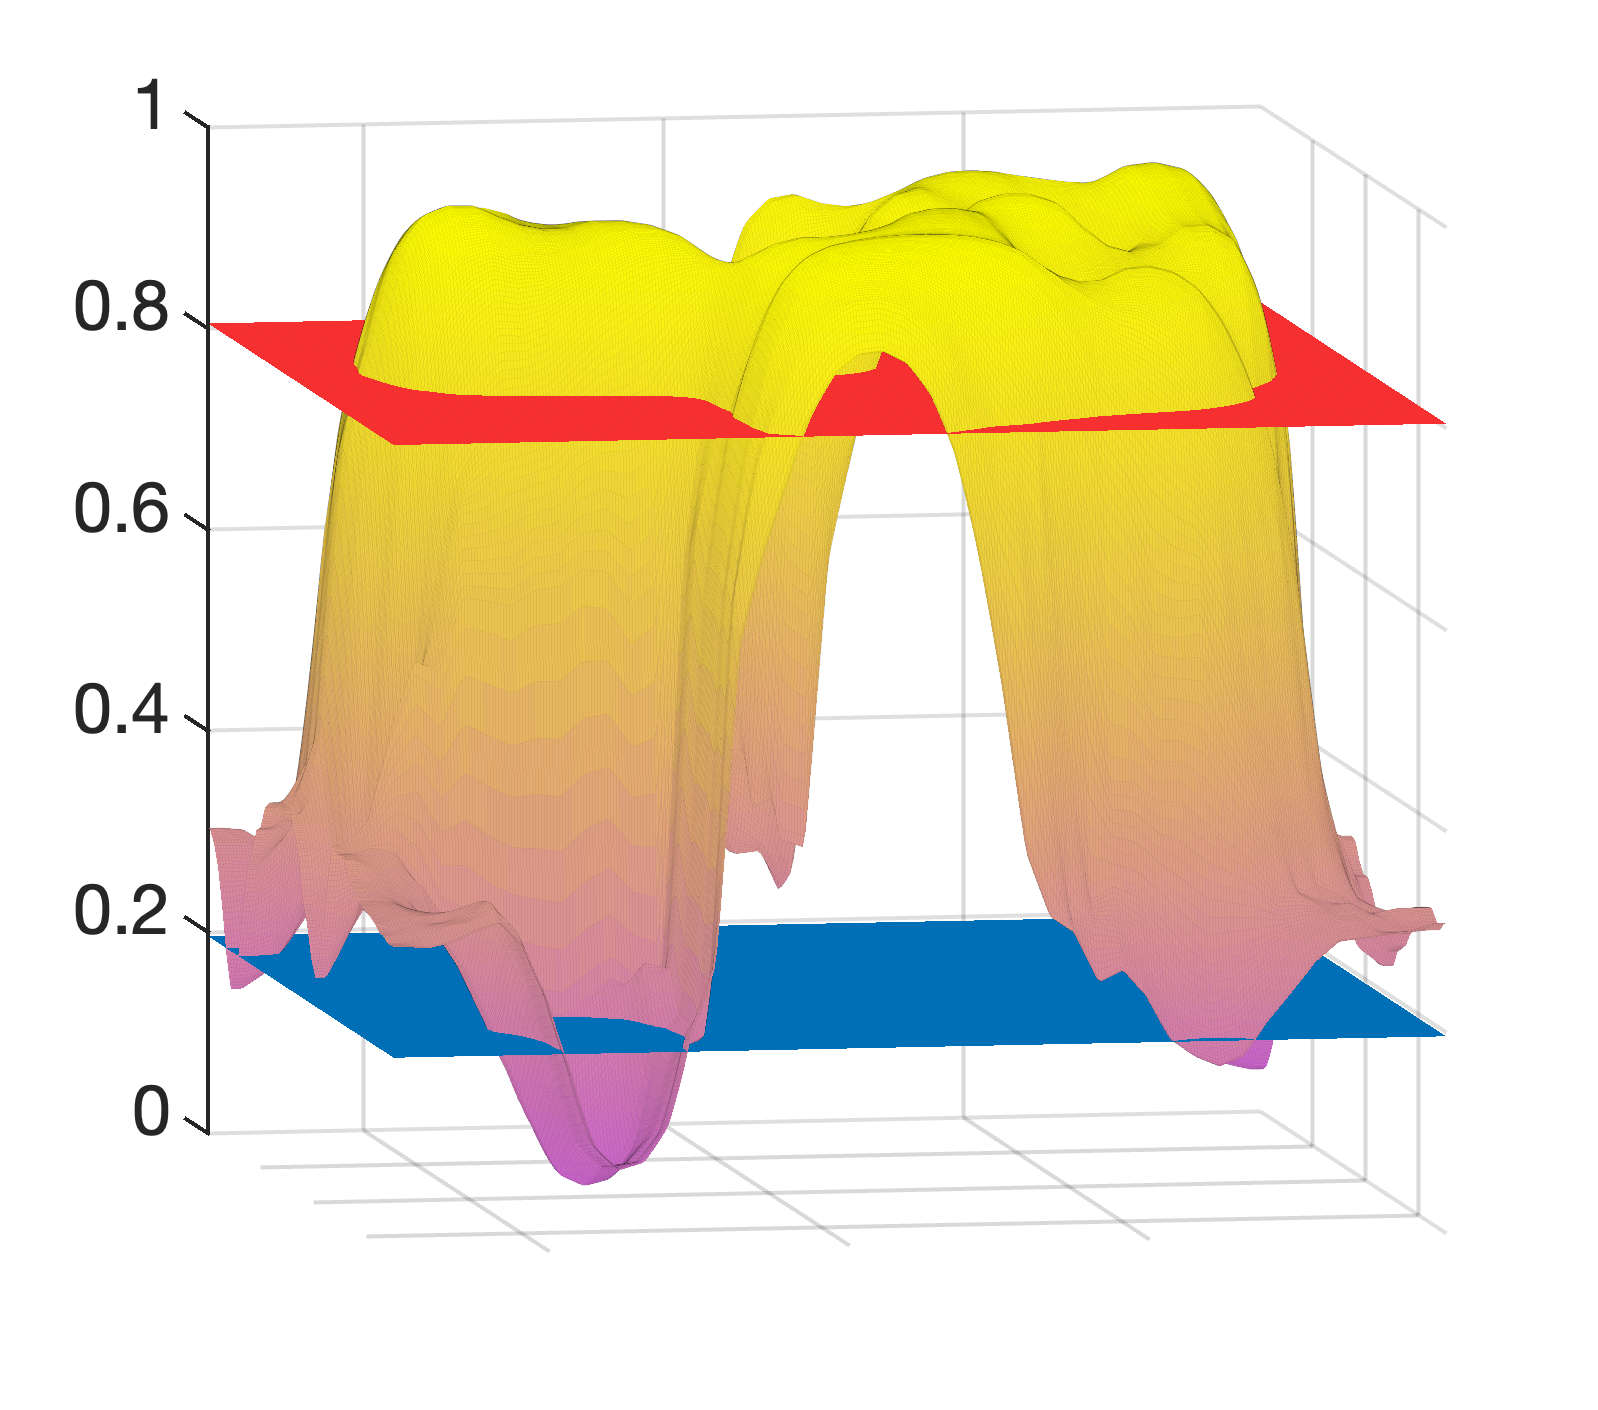
\includegraphics[width=0.24\textwidth]{../figures/learning/score_surf/772.png}	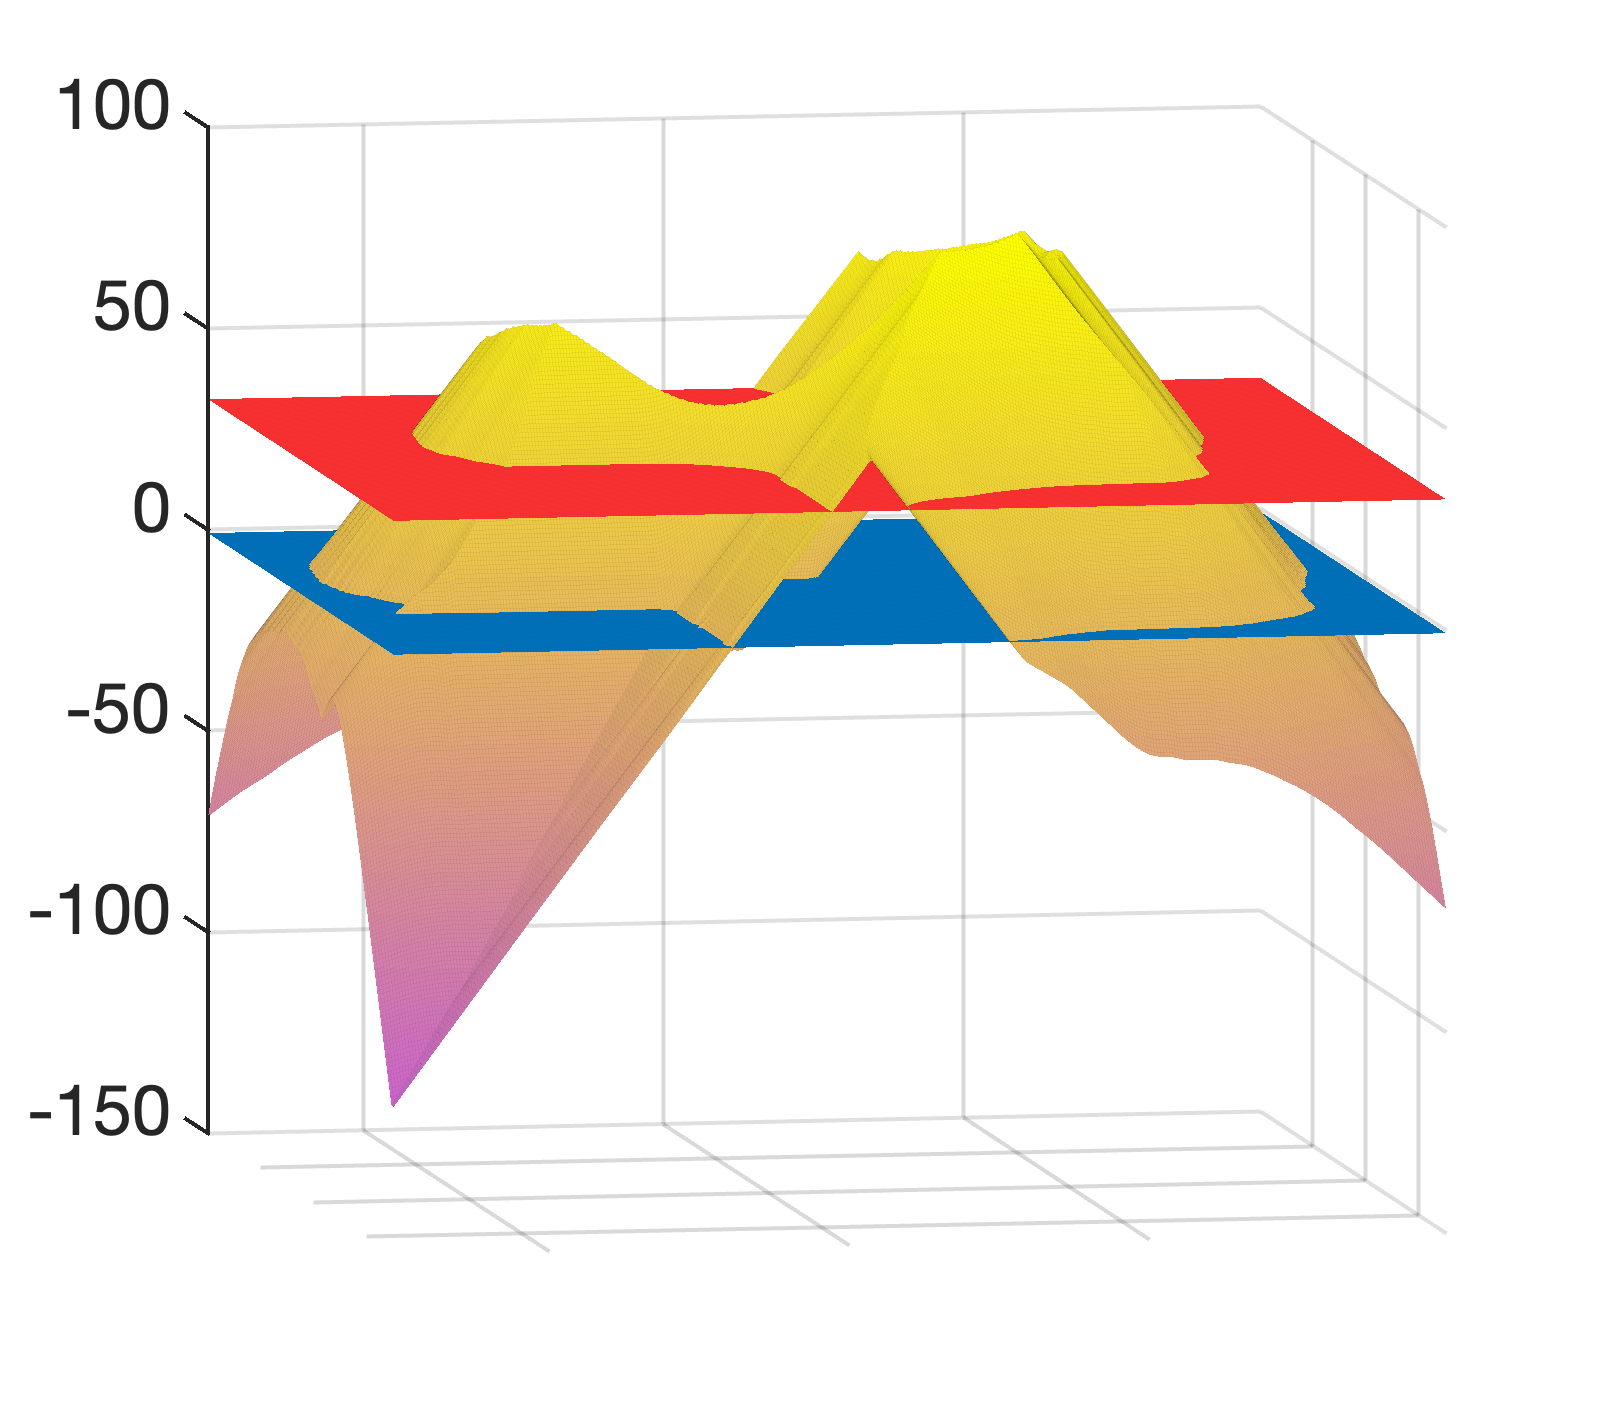
\includegraphics[width=0.24\textwidth]{../figures/learning/dist_surf/772.png}
		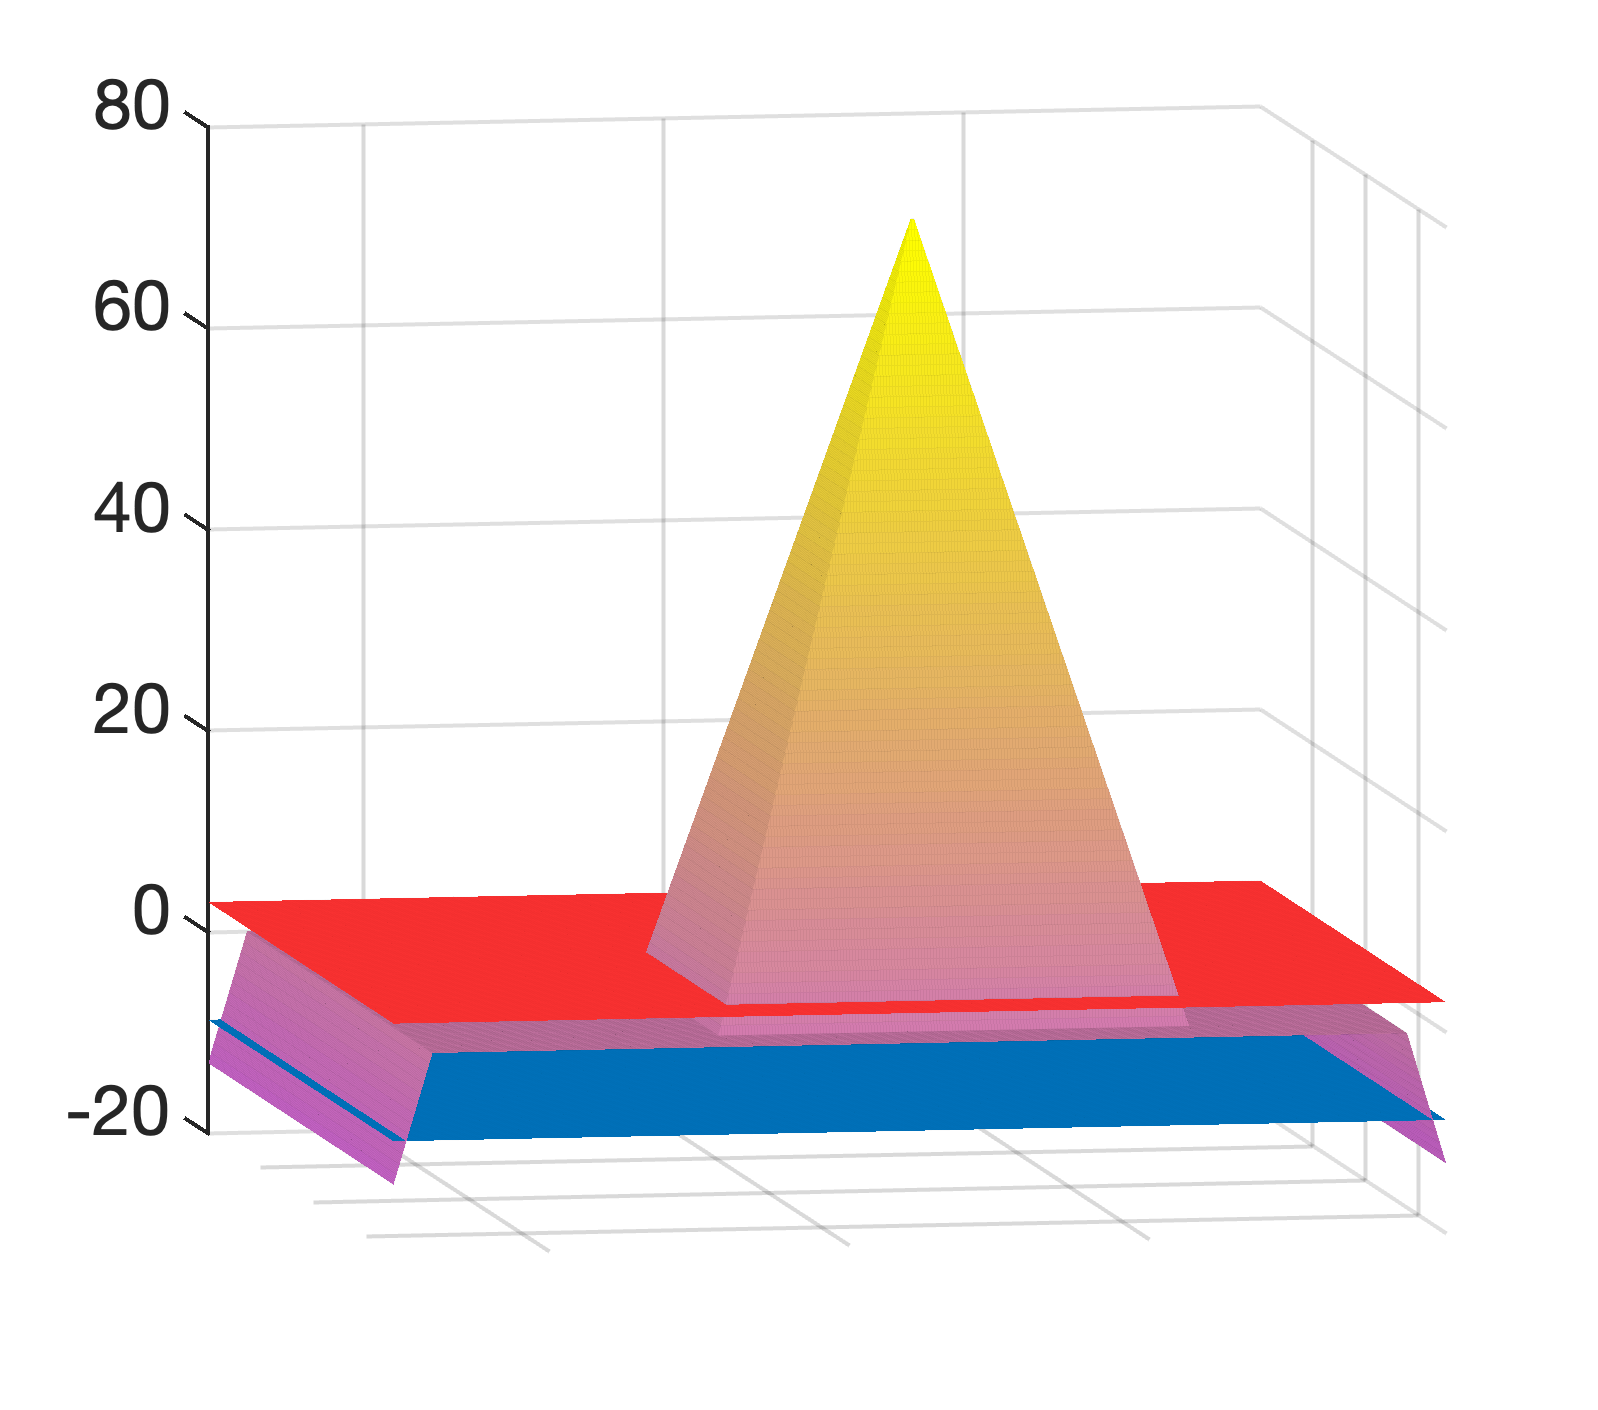
\includegraphics[width=0.24\textwidth]{../figures/learning/dist_bt_surf/772.png}\\
		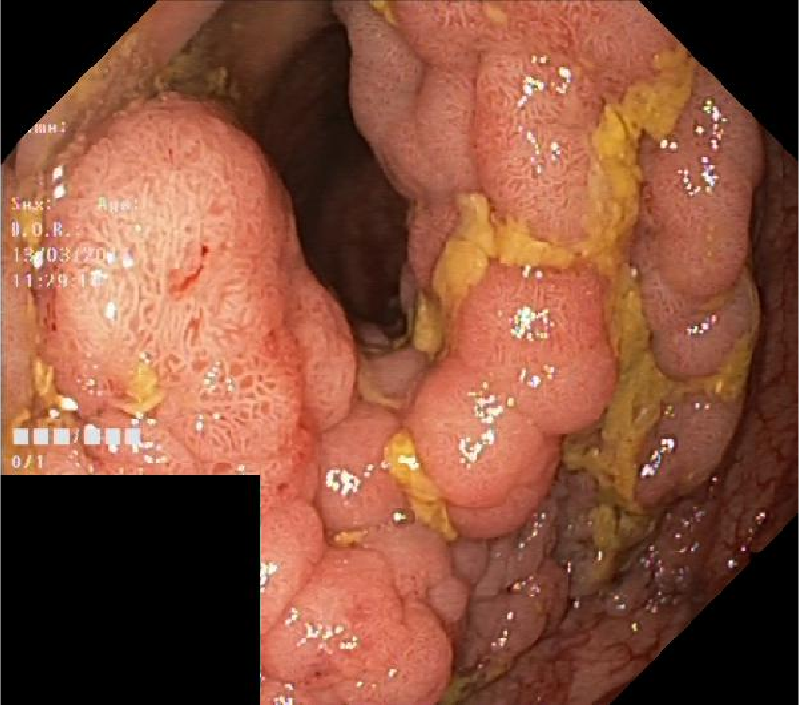
\includegraphics[width=0.24\textwidth]{../figures/learning/images/772.png}
		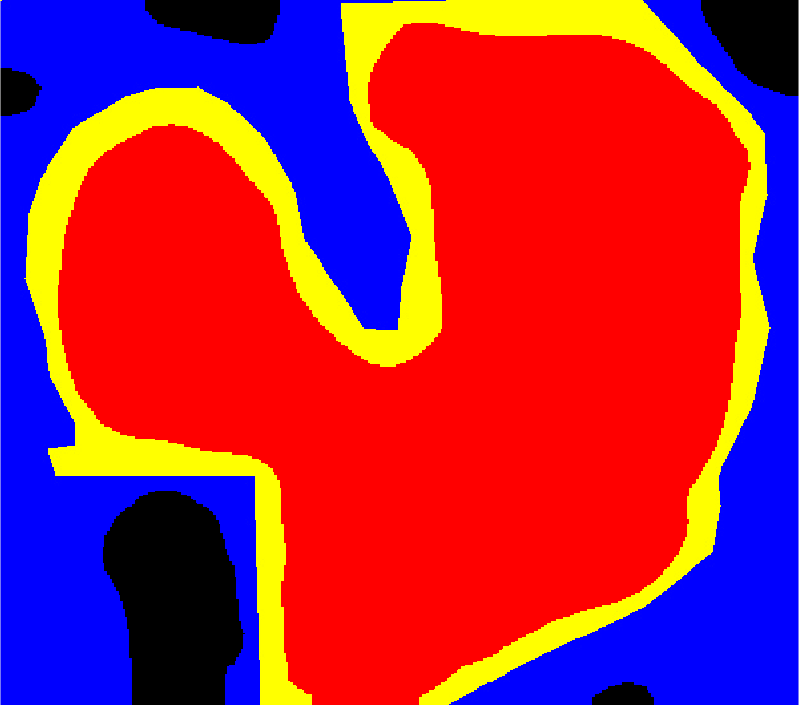
\includegraphics[width=0.24\textwidth]{../figures/learning/score_crs_marginal90/772.png}
		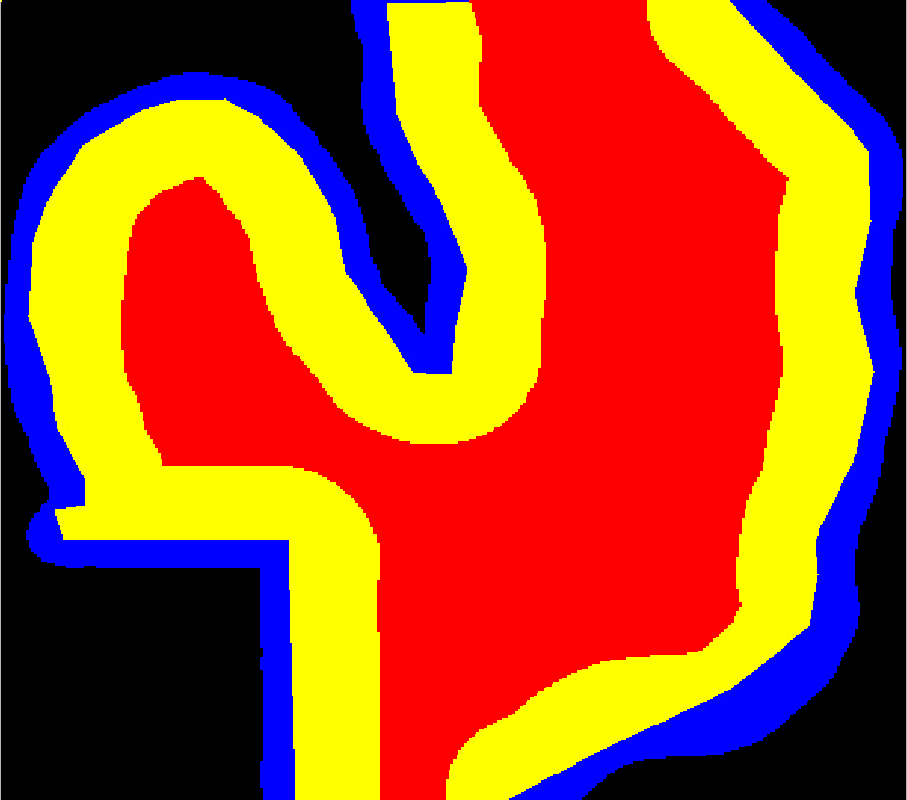
\includegraphics[width=0.24\textwidth]{../figures/learning/dist_crs_marginal90/772.png}
		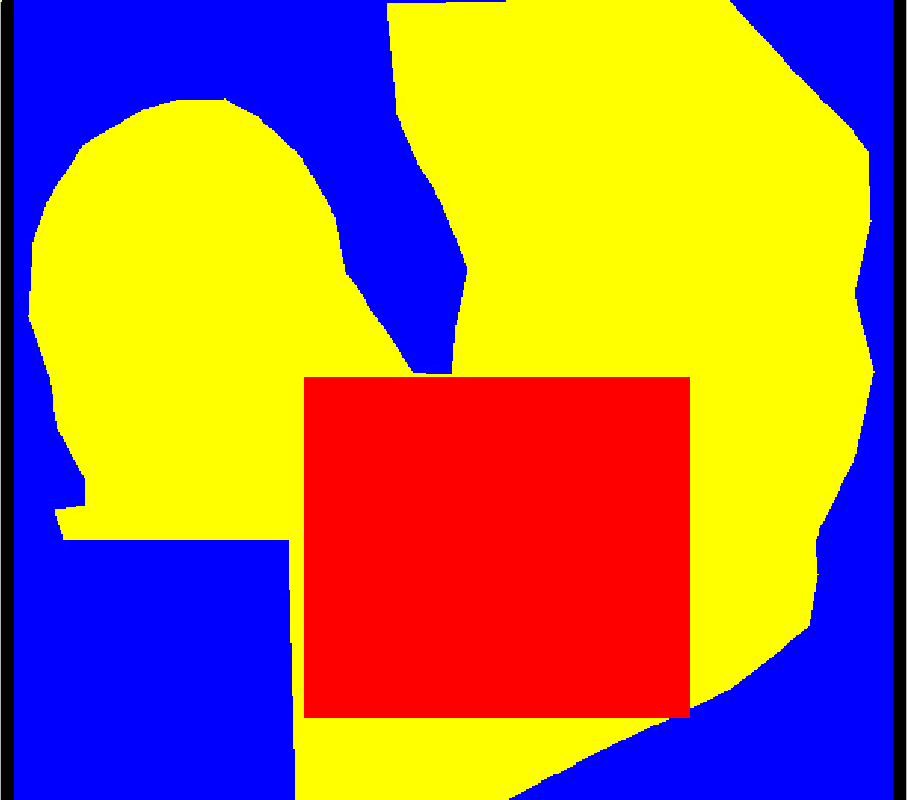
\includegraphics[width=0.24\textwidth]{../figures/learning/dist_bt_crs_marginal90/772.png}\\
		\vspace{0.5cm}
		
\includegraphics[width=0.24\textwidth]{../figures/learning/scores/202.png}
		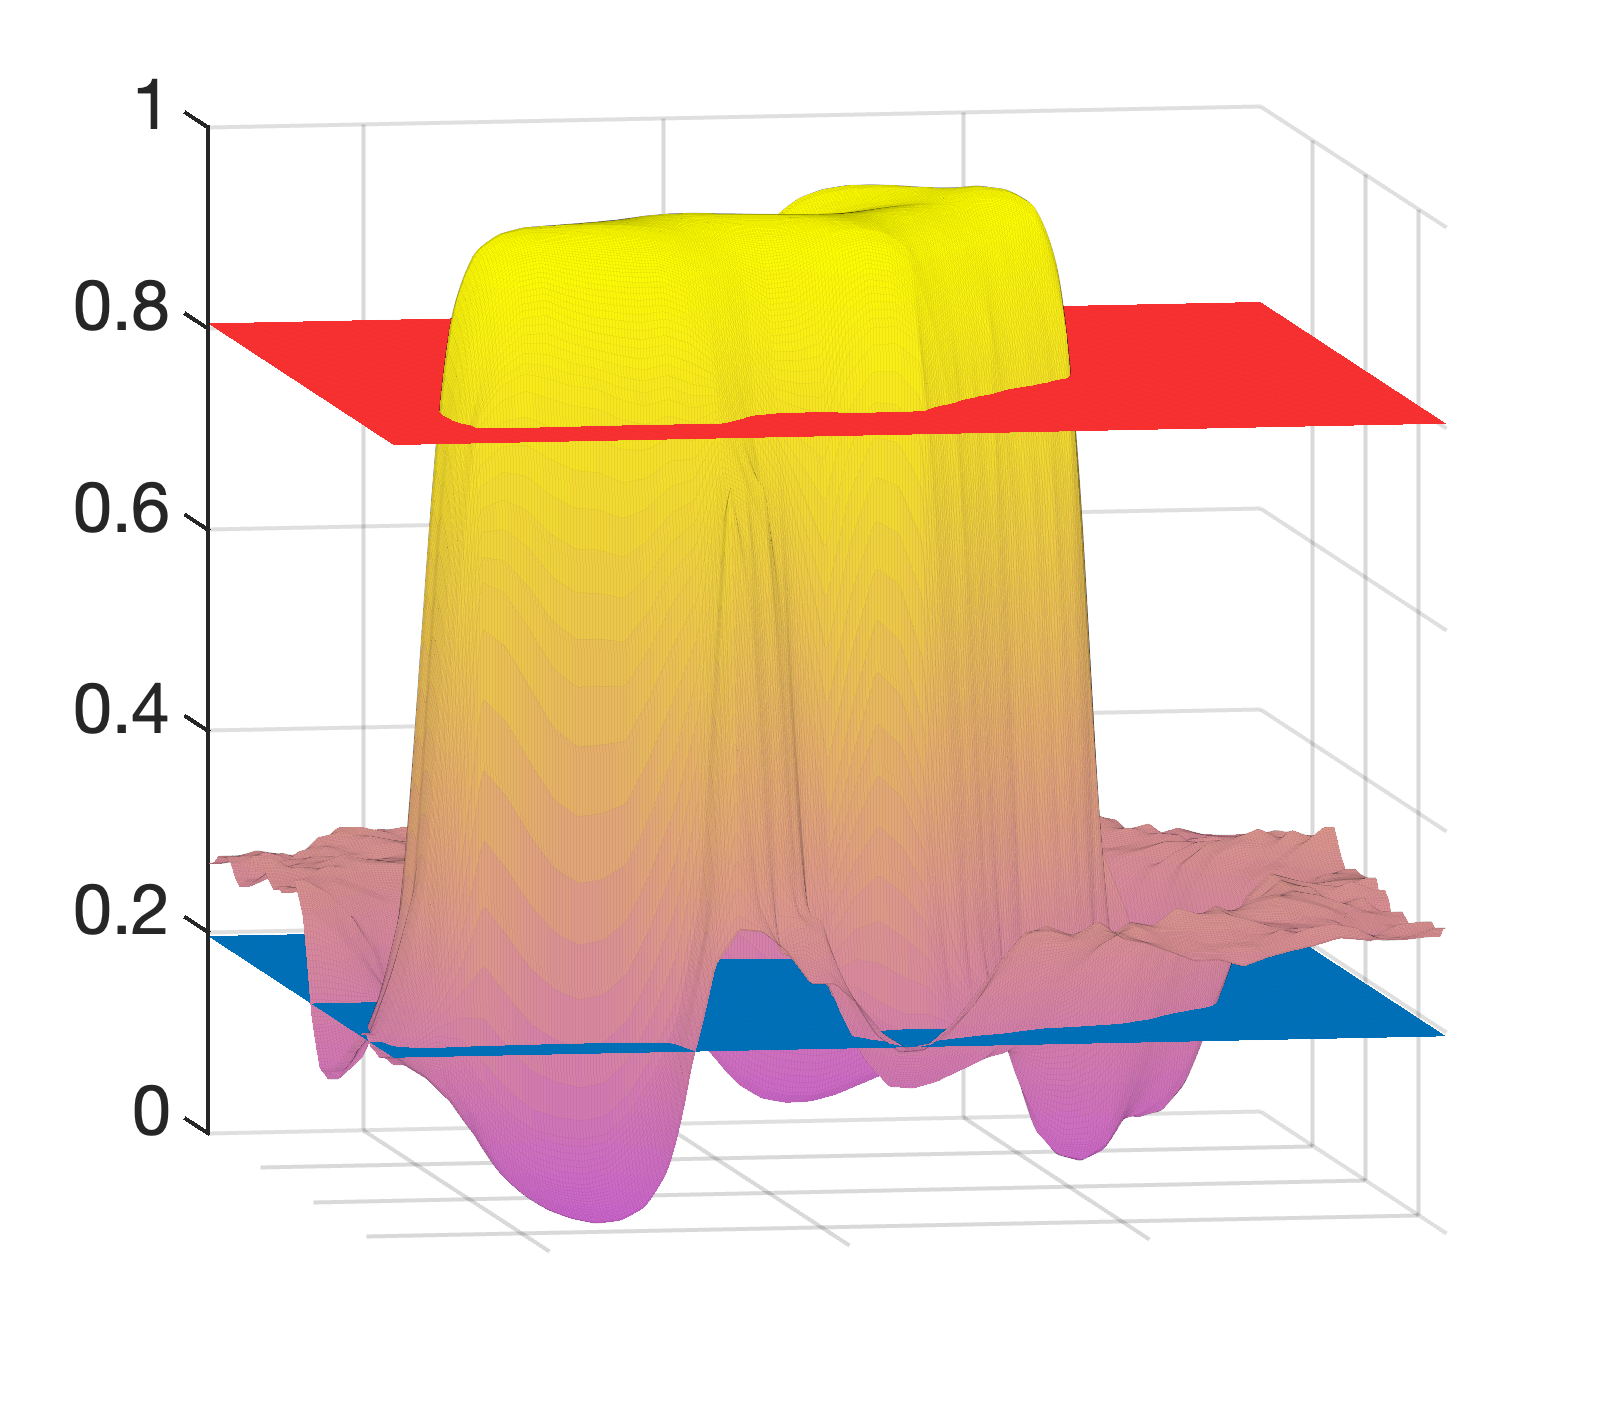
\includegraphics[width=0.24\textwidth]{../figures/learning/score_surf/202.png}	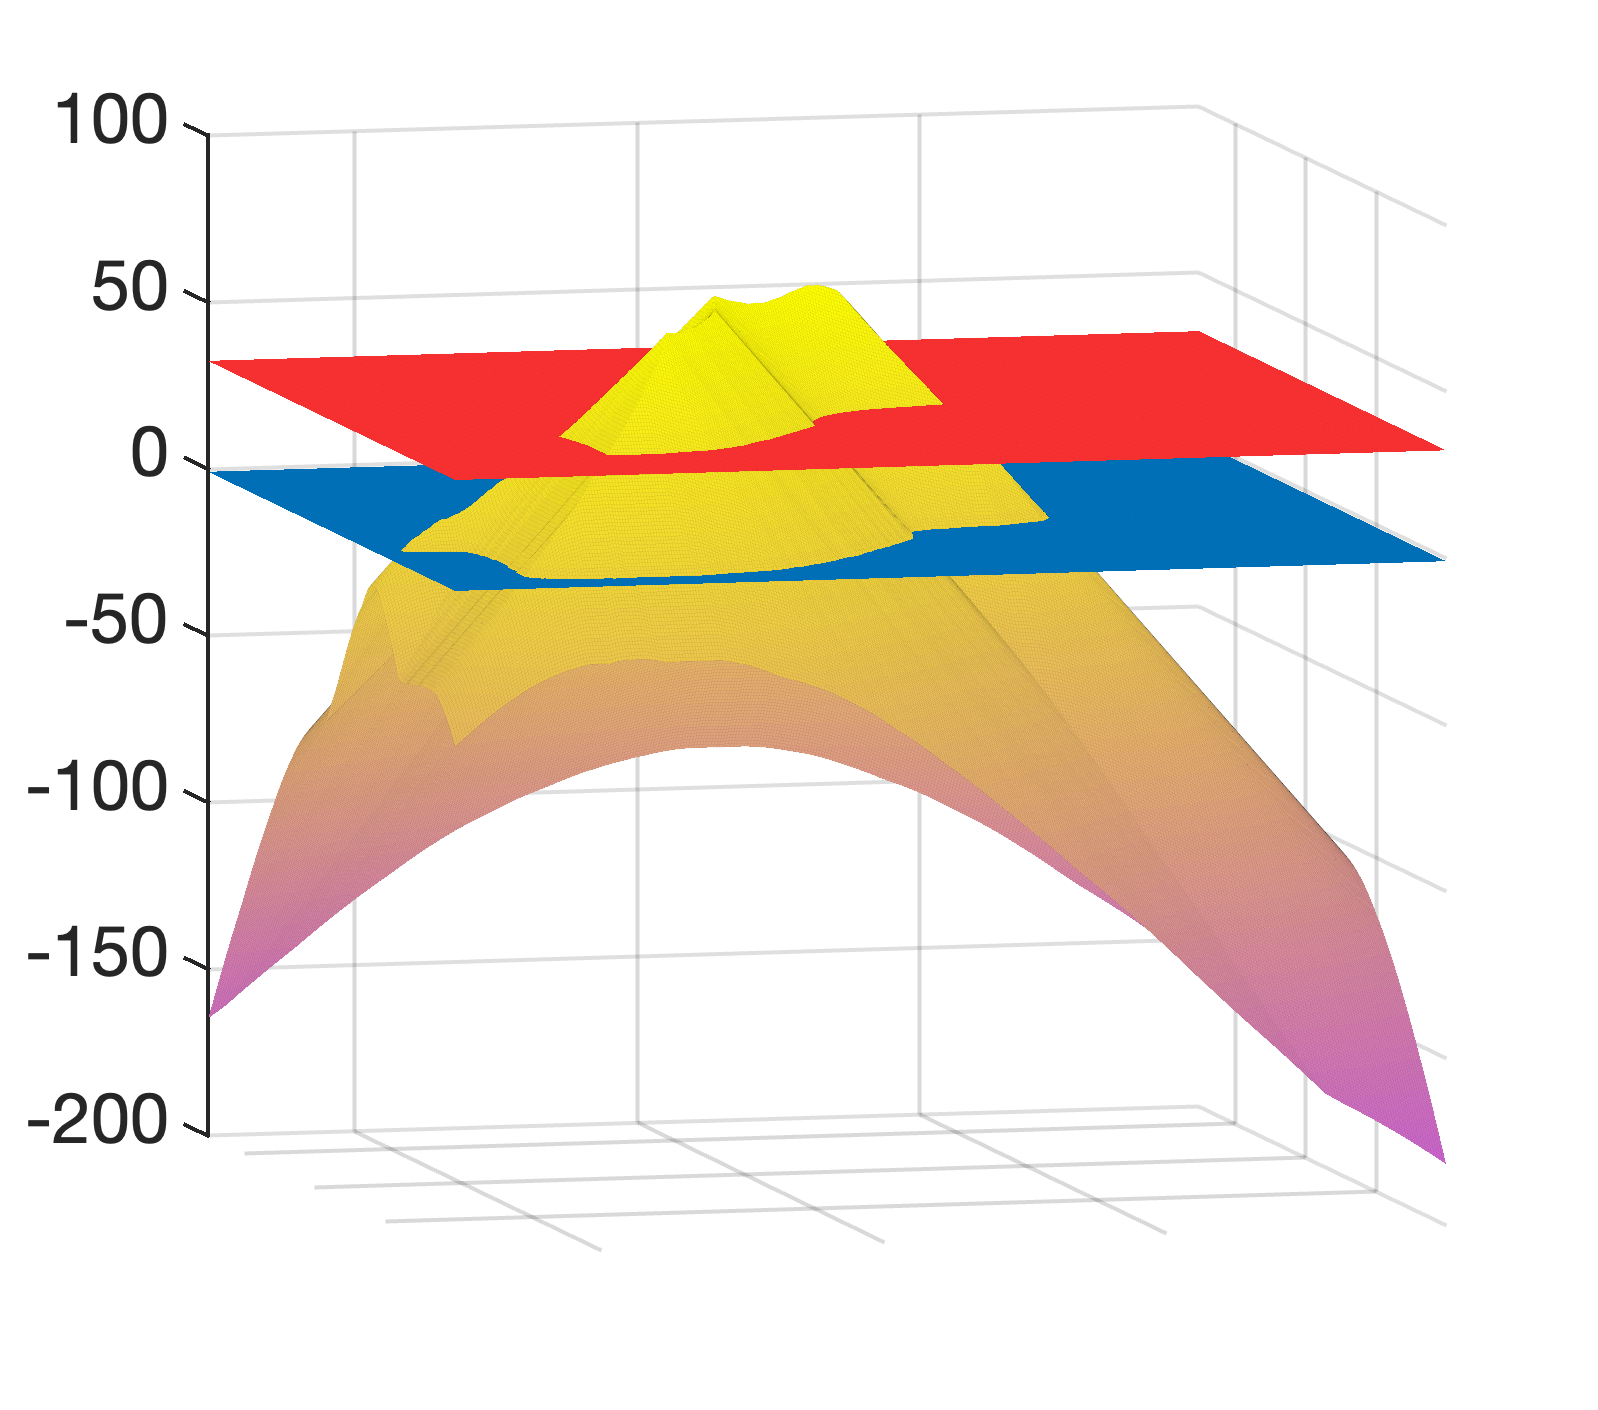
\includegraphics[width=0.24\textwidth]{../figures/learning/dist_surf/202.png}
		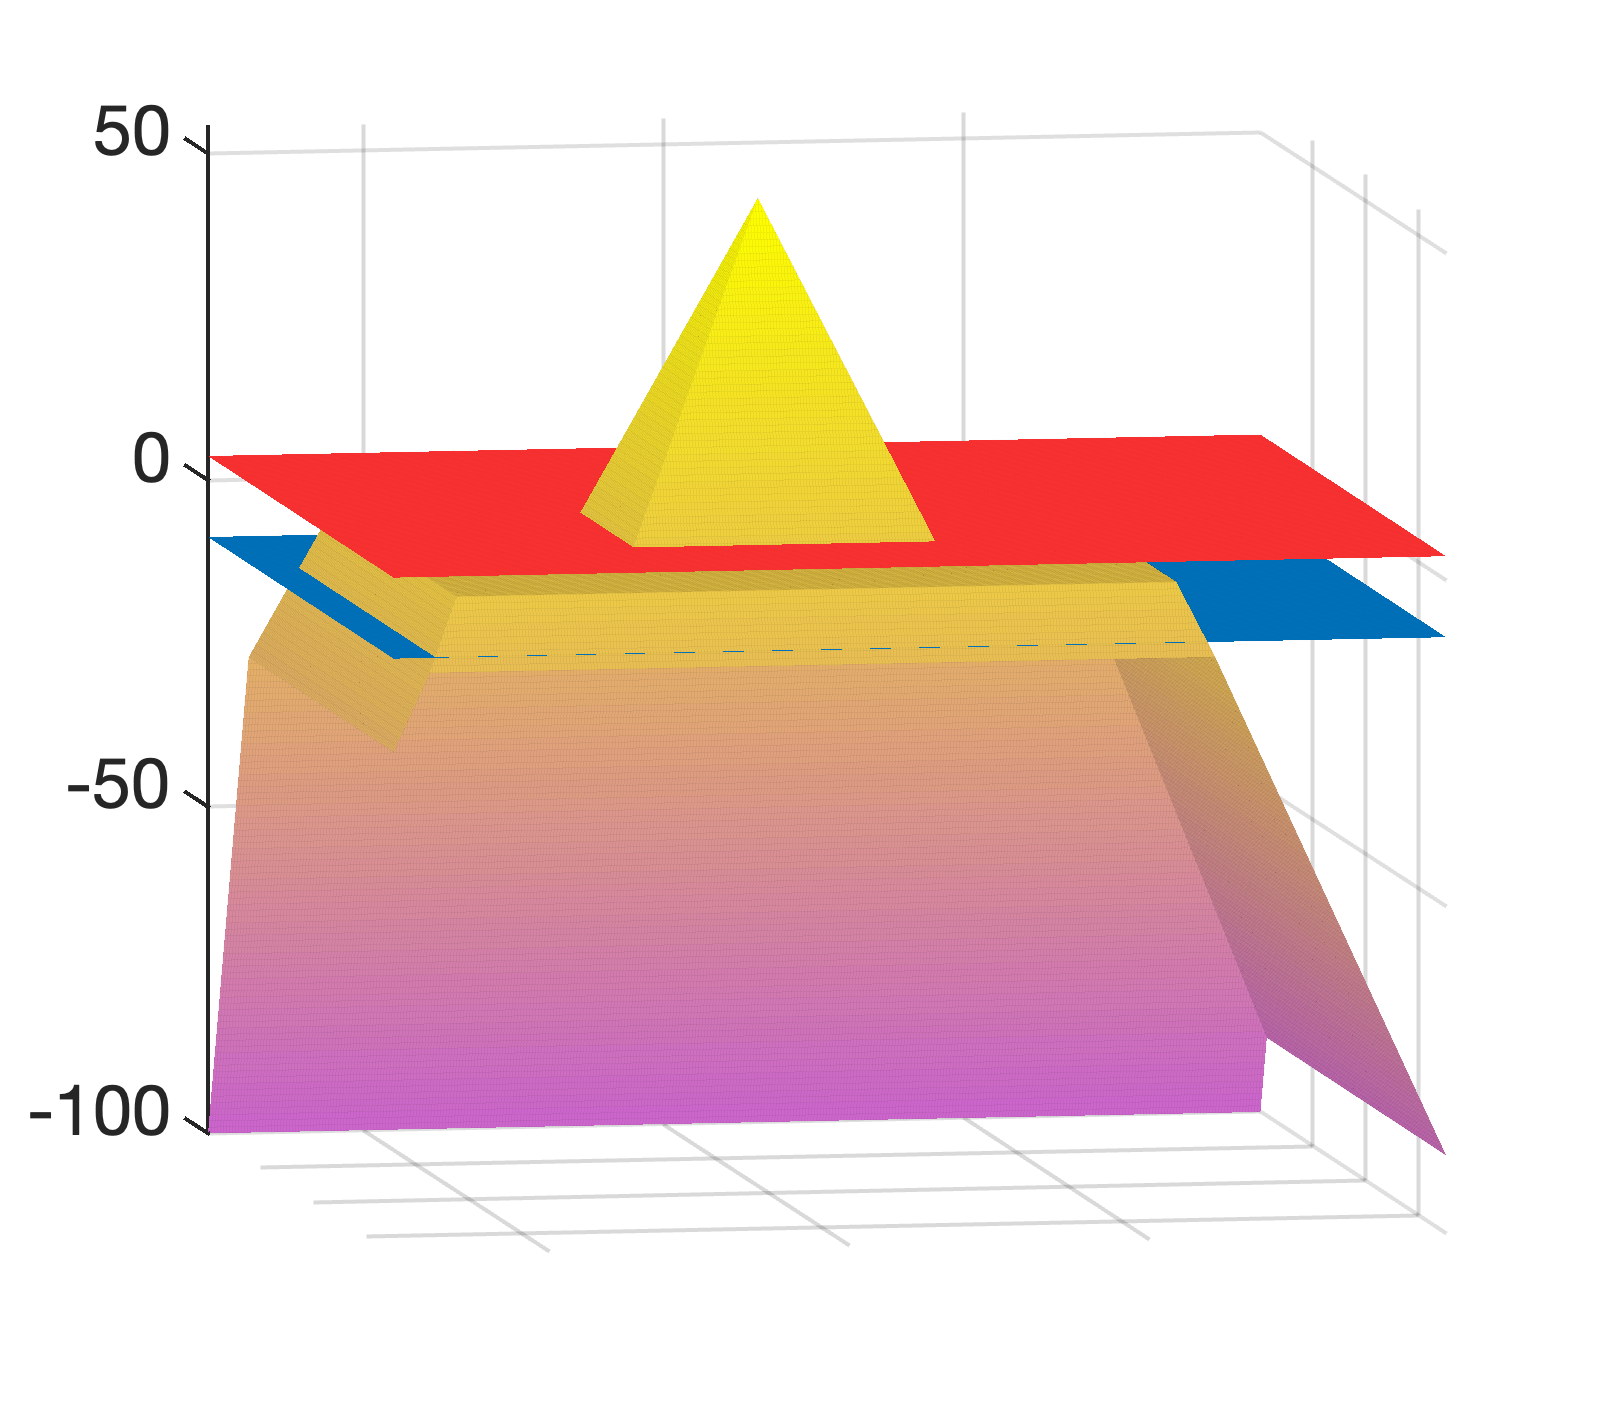
\includegraphics[width=0.24\textwidth]{../figures/learning/dist_bt_surf/202.png}\\
		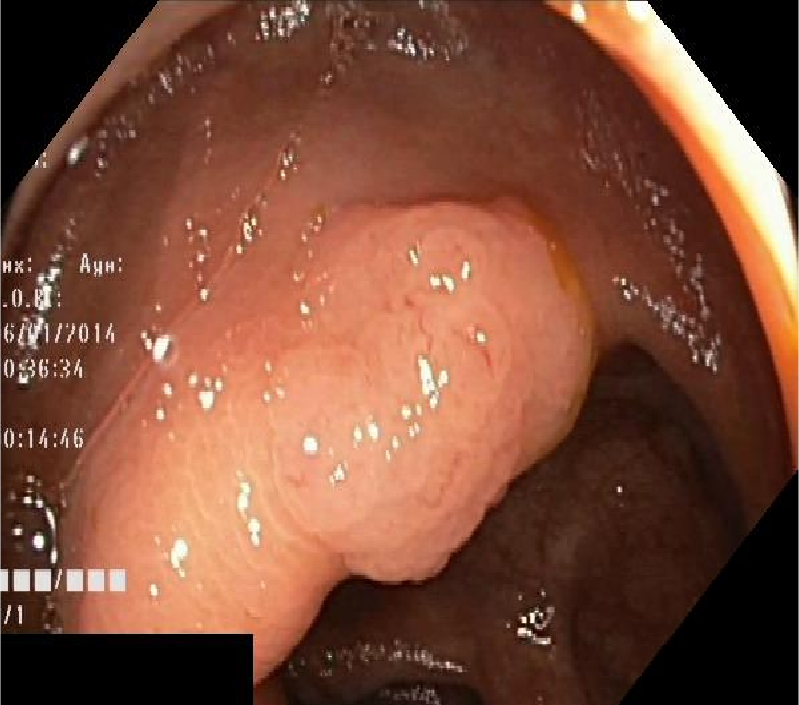
\includegraphics[width=0.24\textwidth]{../figures/learning/images/202.png}
		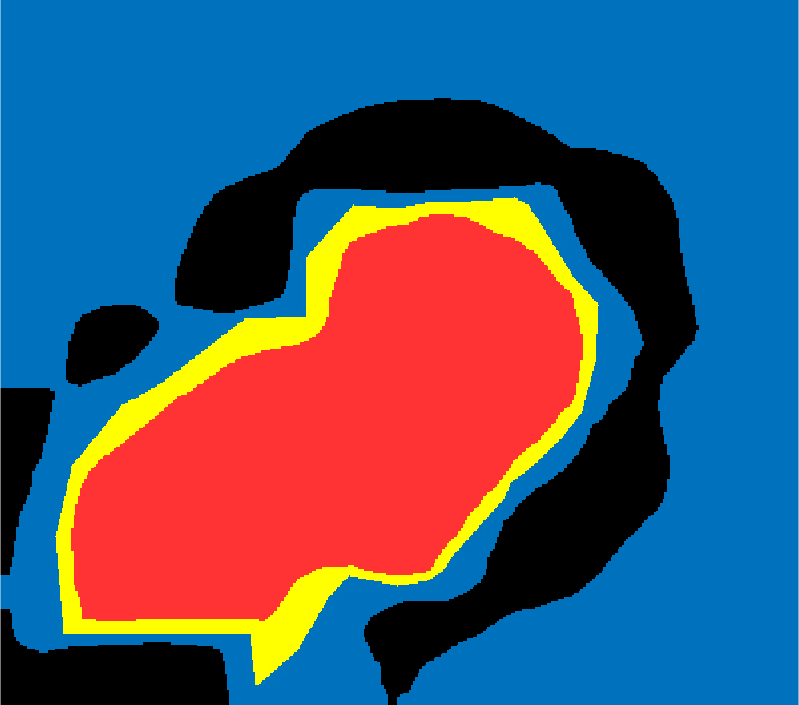
\includegraphics[width=0.24\textwidth]{../figures/learning/score_crs_marginal90/202.png}
		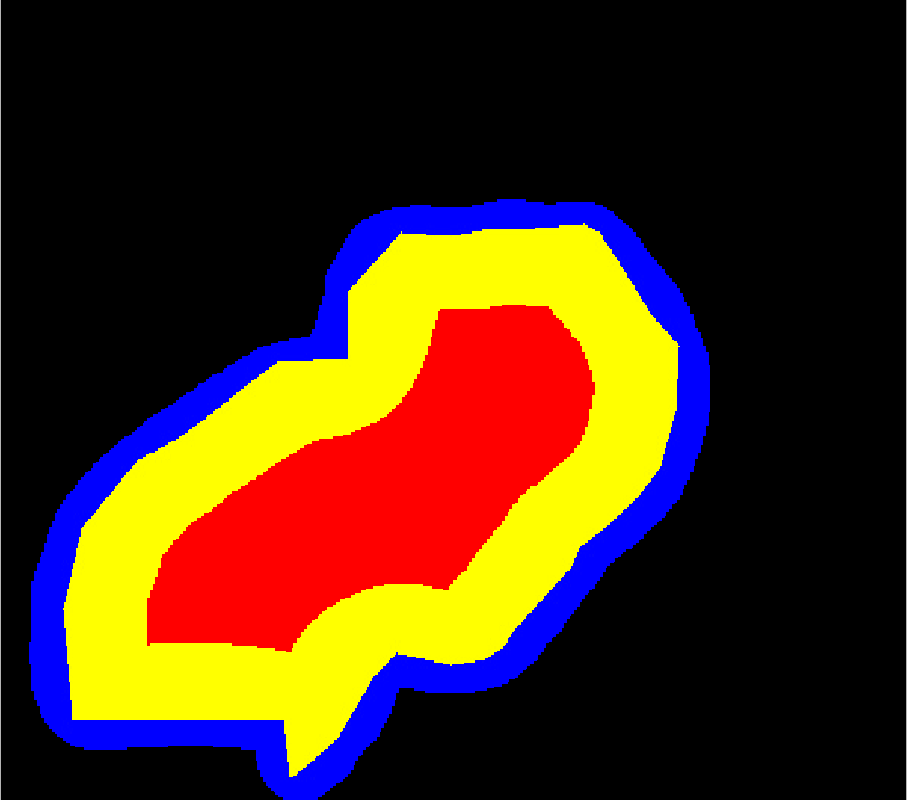
\includegraphics[width=0.24\textwidth]{../figures/learning/dist_crs_marginal90/202.png}
		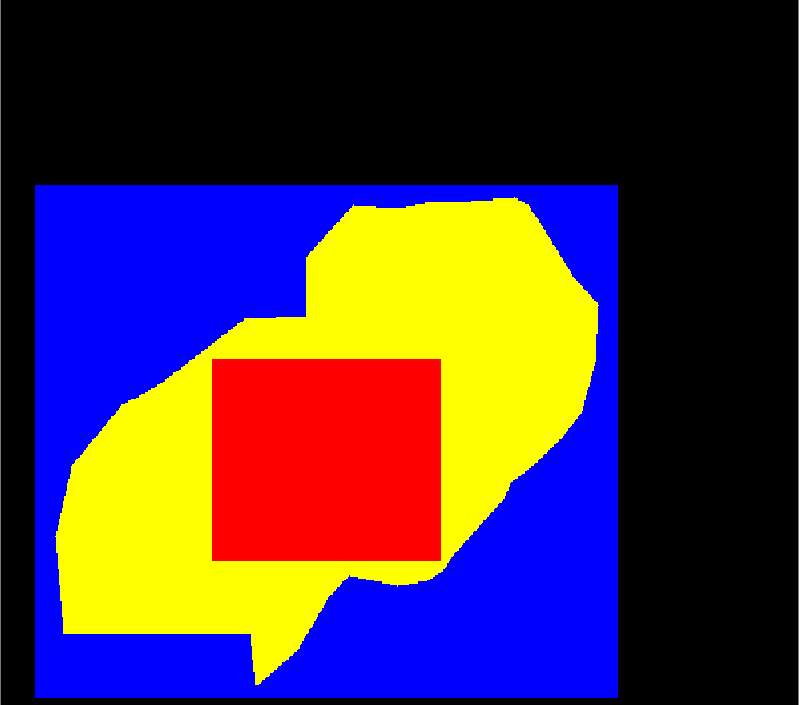
\includegraphics[width=0.24\textwidth]{../figures/learning/dist_bt_crs_marginal90/202.png}\\
			\vspace{0.5cm}
		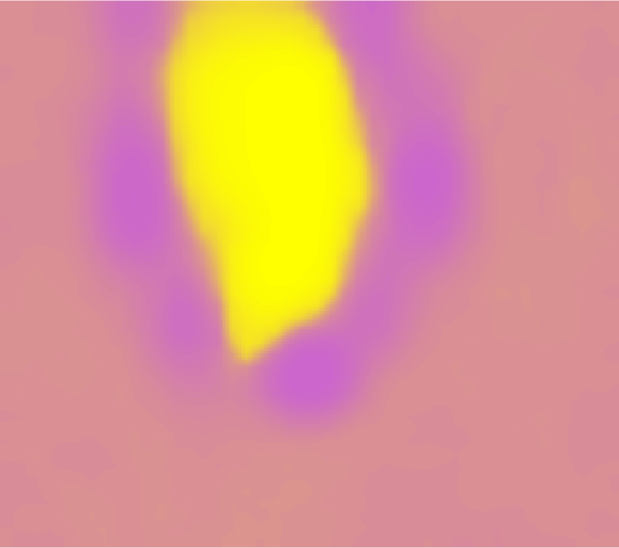
\includegraphics[width=0.24\textwidth]{../figures/learning/scores/54.png}
		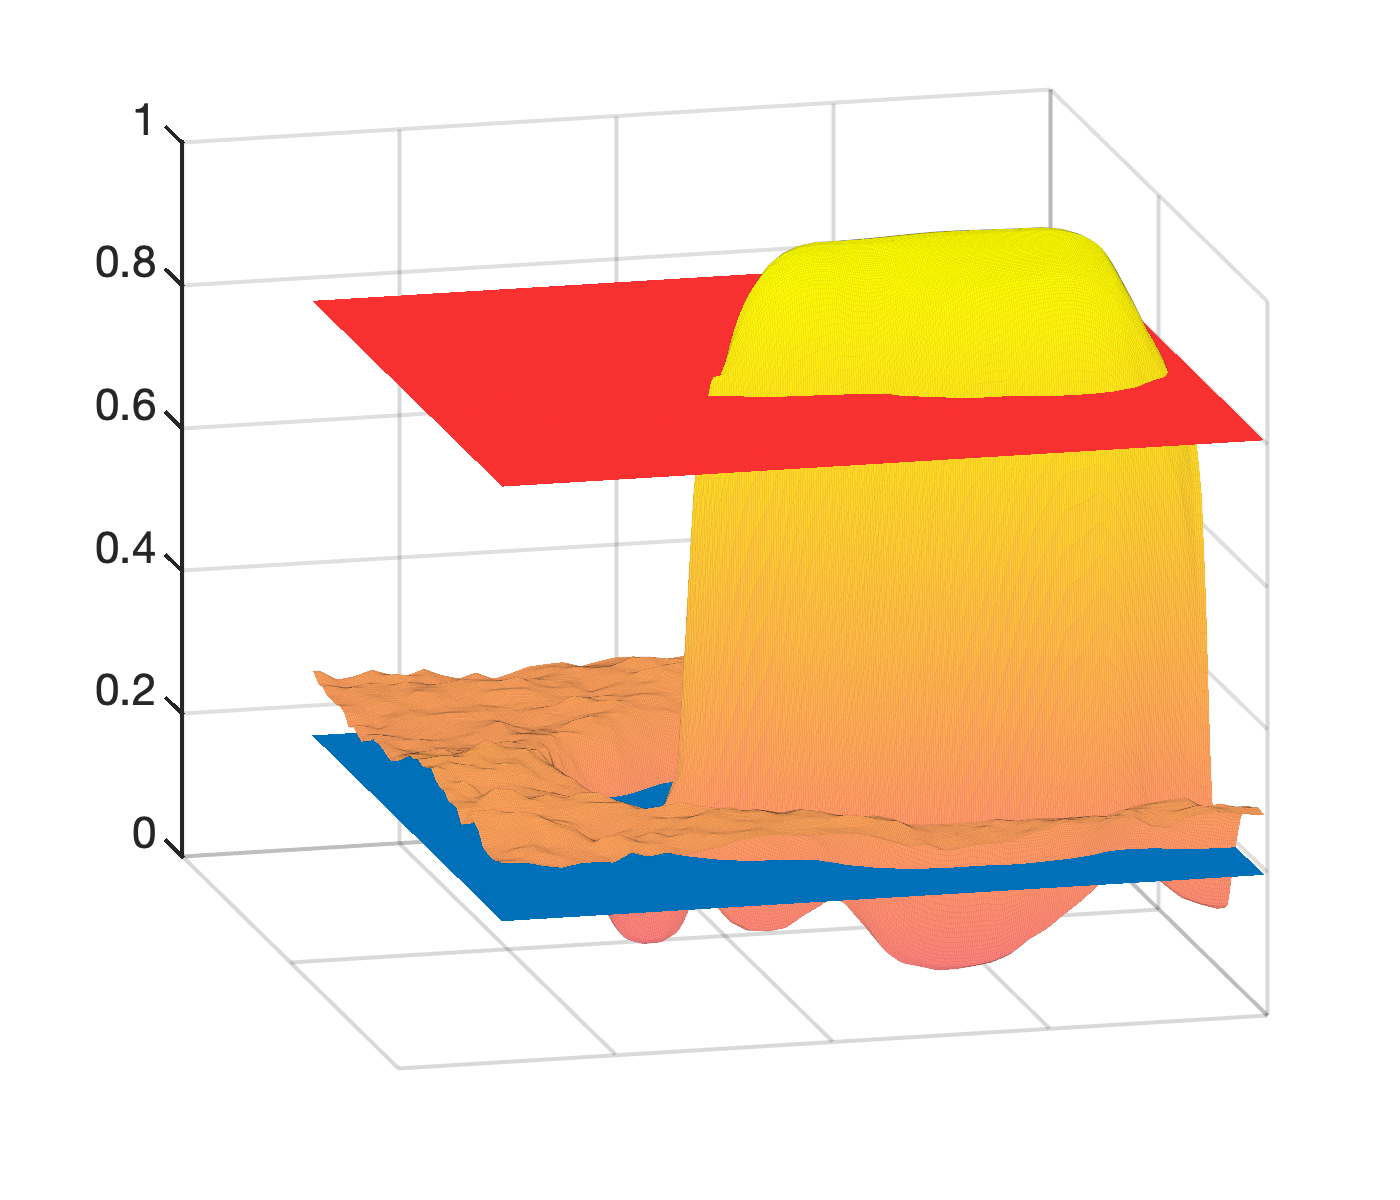
\includegraphics[width=0.24\textwidth]{../figures/learning/score_surf/54.png}	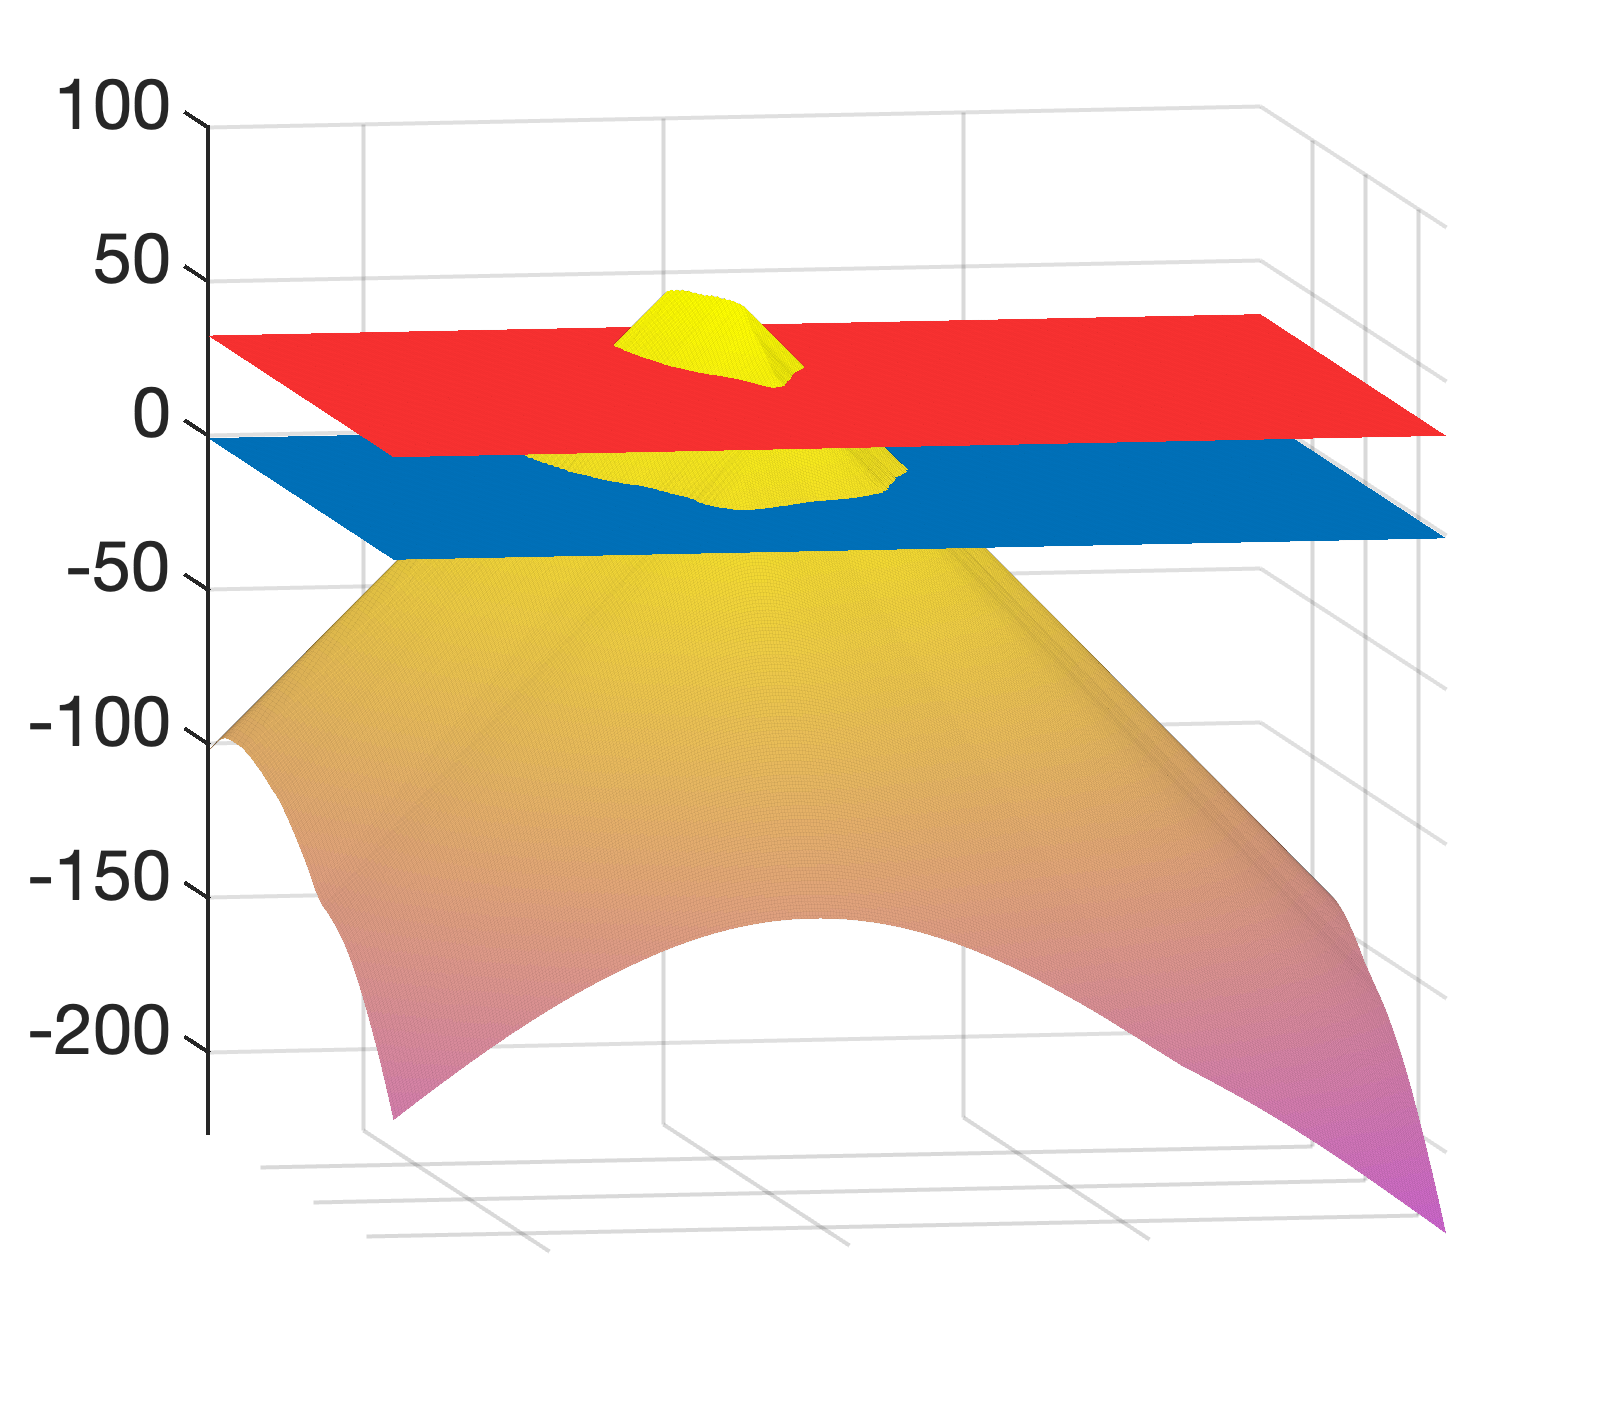
\includegraphics[width=0.24\textwidth]{../figures/learning/dist_surf/54.png}
		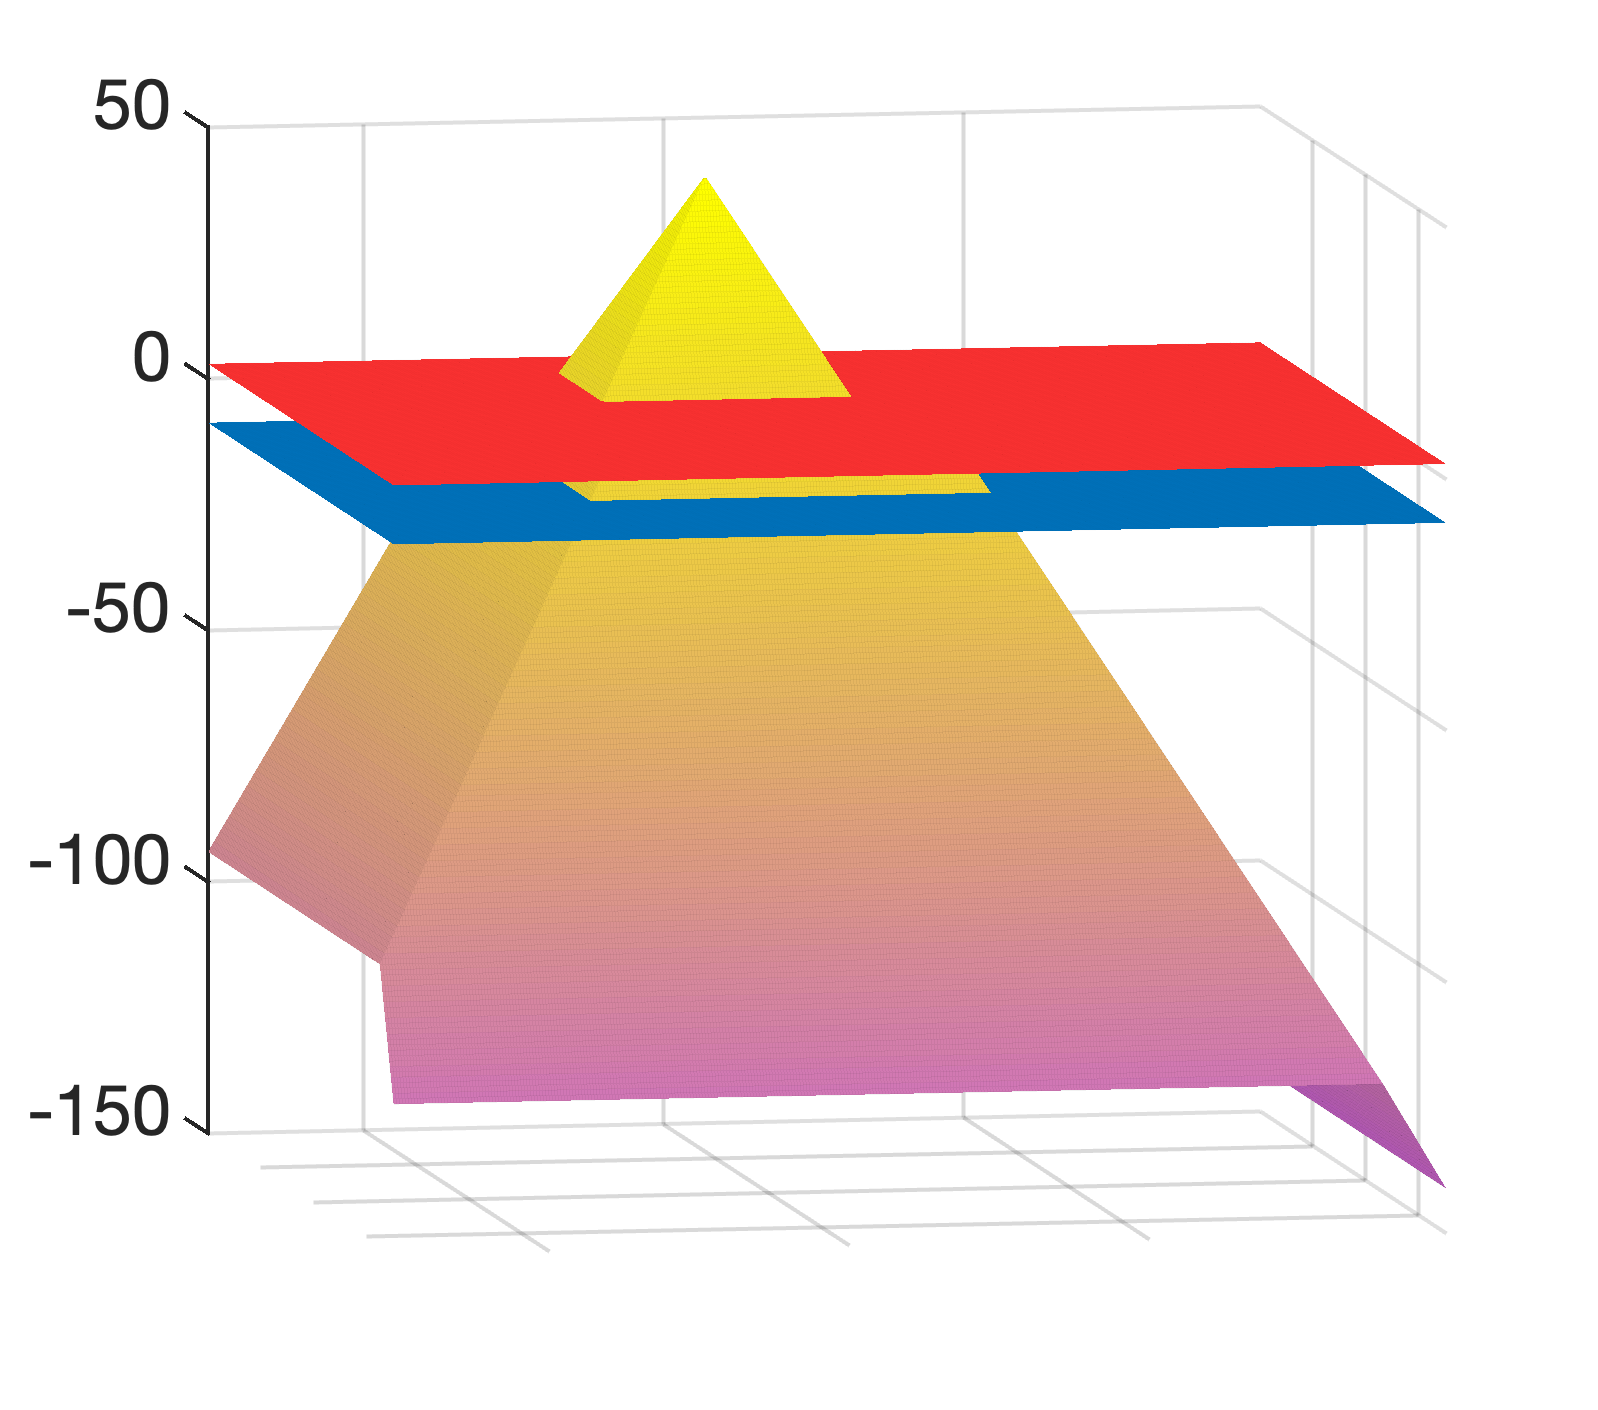
\includegraphics[width=0.24\textwidth]{../figures/learning/dist_bt_surf/54.png}\\
		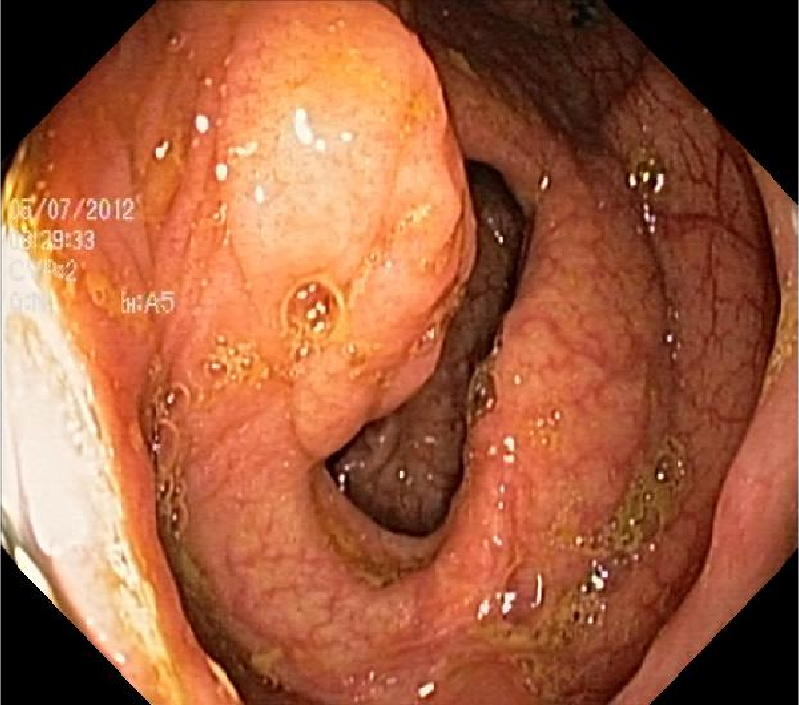
\includegraphics[width=0.24\textwidth]{../figures/learning/images/54.png}
		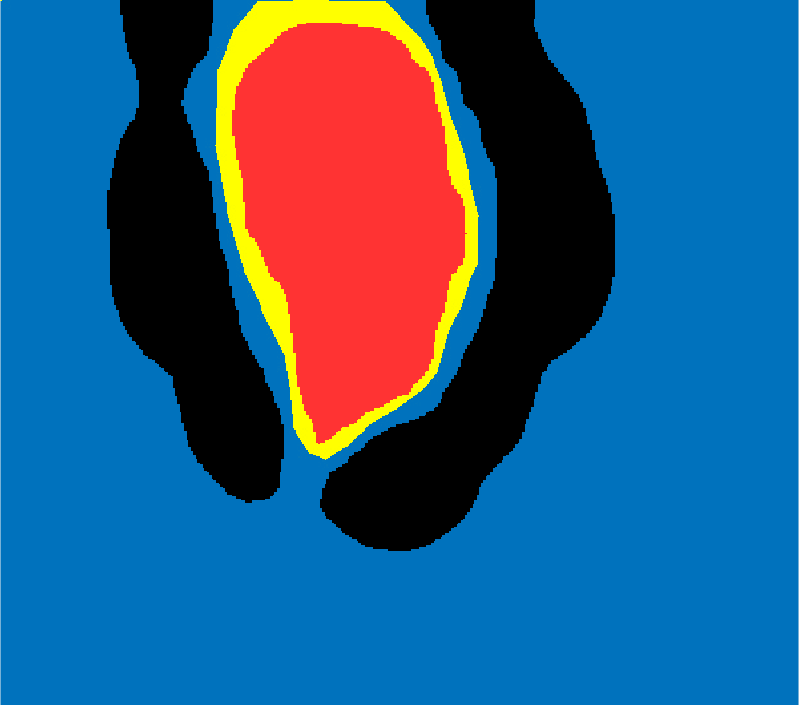
\includegraphics[width=0.24\textwidth]{../figures/learning/score_crs_marginal90/54.png}
		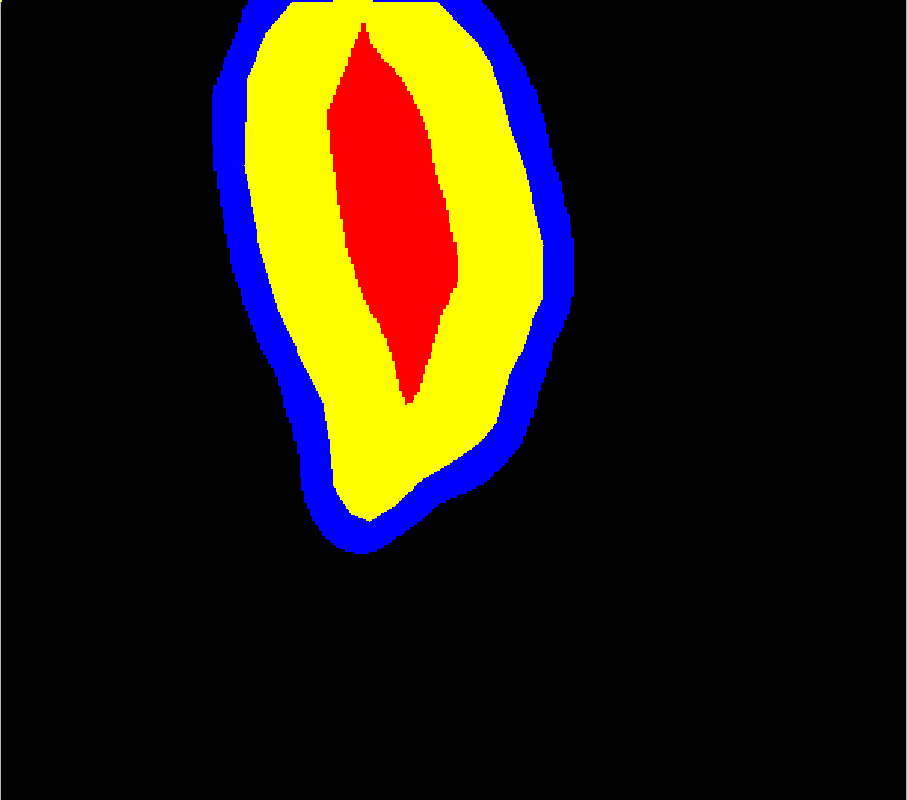
\includegraphics[width=0.24\textwidth]{../figures/learning/dist_crs_marginal90/54.png}
		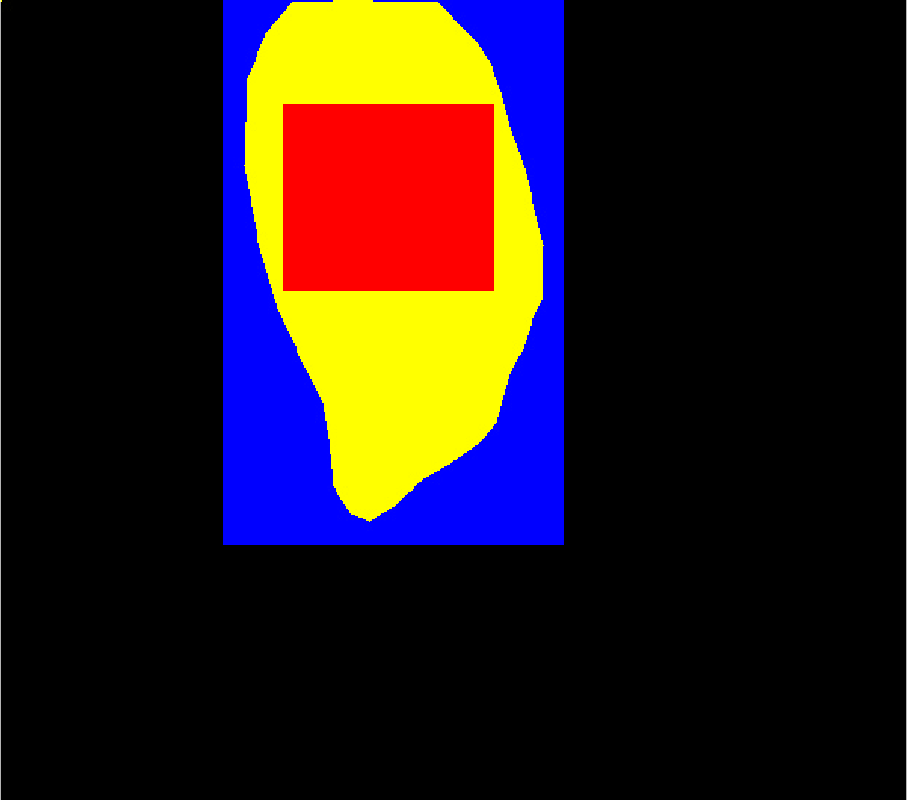
\includegraphics[width=0.24\textwidth]{../figures/learning/dist_bt_crs_marginal90/54.png}
	\end{center}
	\caption{Additional examples from the learning dataset. The layout of these figures is the same as for Figure \ref{fig:learning}.}
	\label{fig:learning2}
\end{figure}

\begin{figure}
	%	\centering
	\begin{center}
		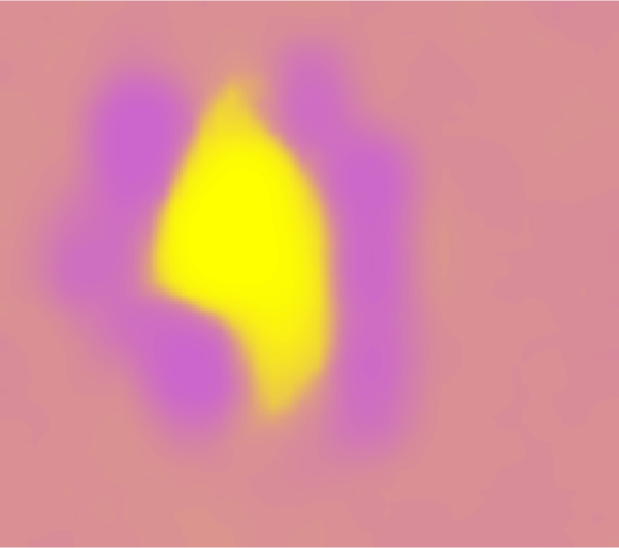
\includegraphics[width=0.24\textwidth]{../figures/learning/scores/183.png}
		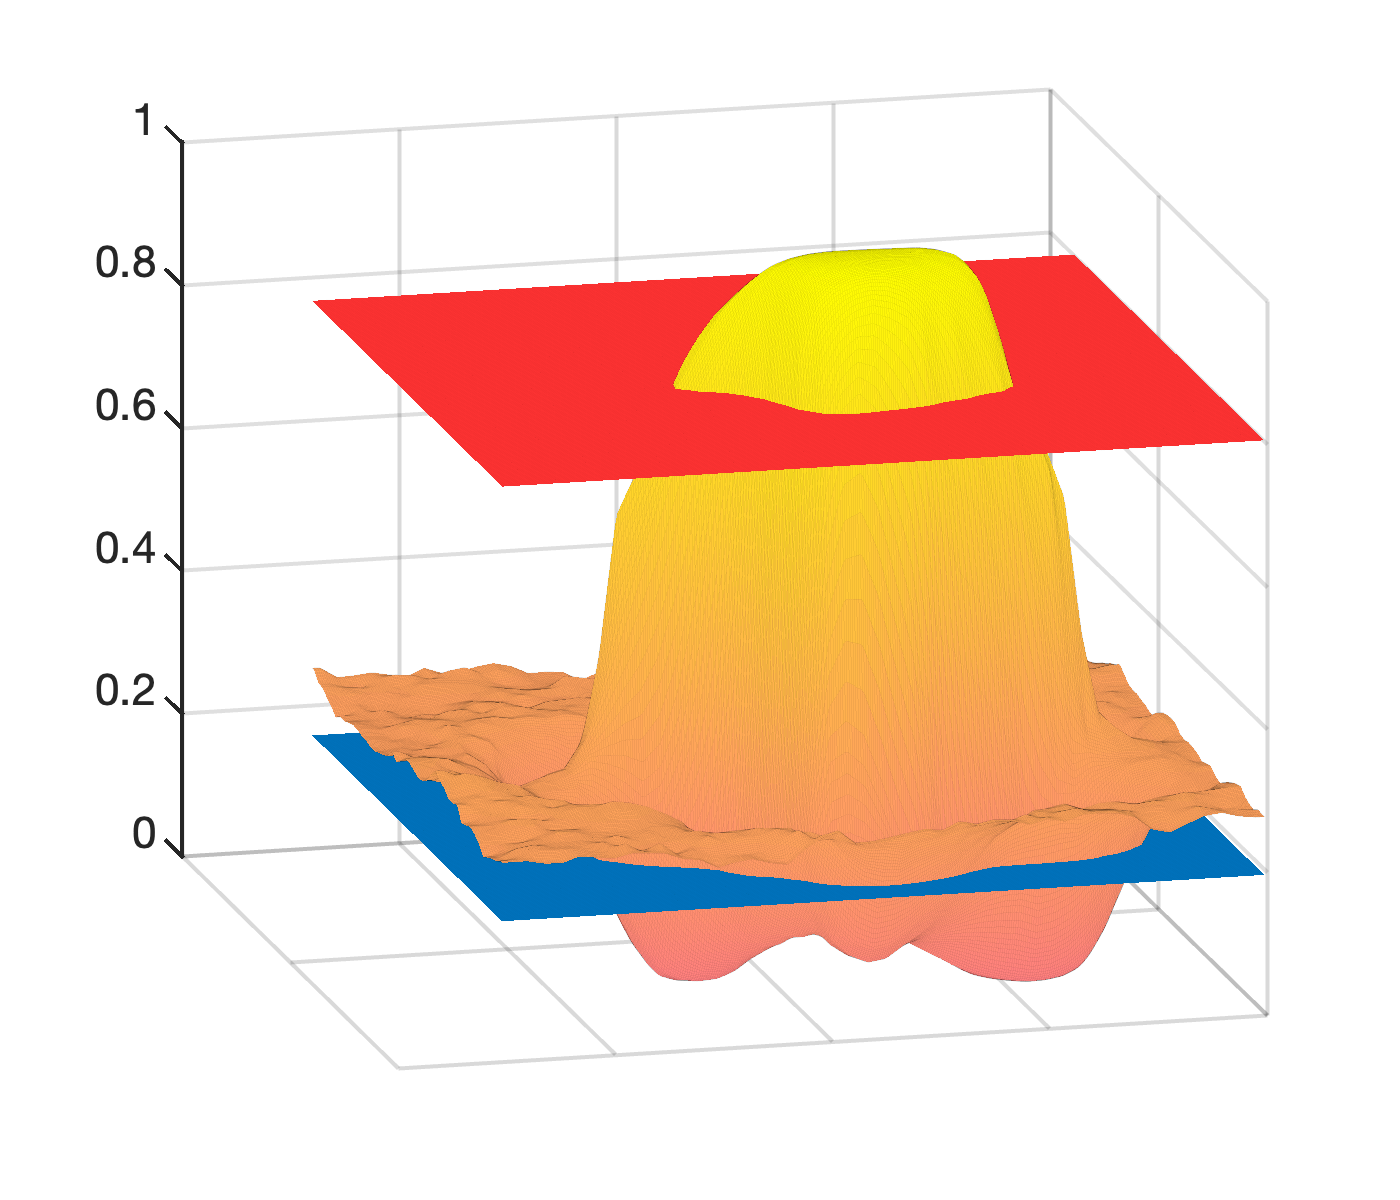
\includegraphics[width=0.24\textwidth]{../figures/learning/score_surf/183.png}	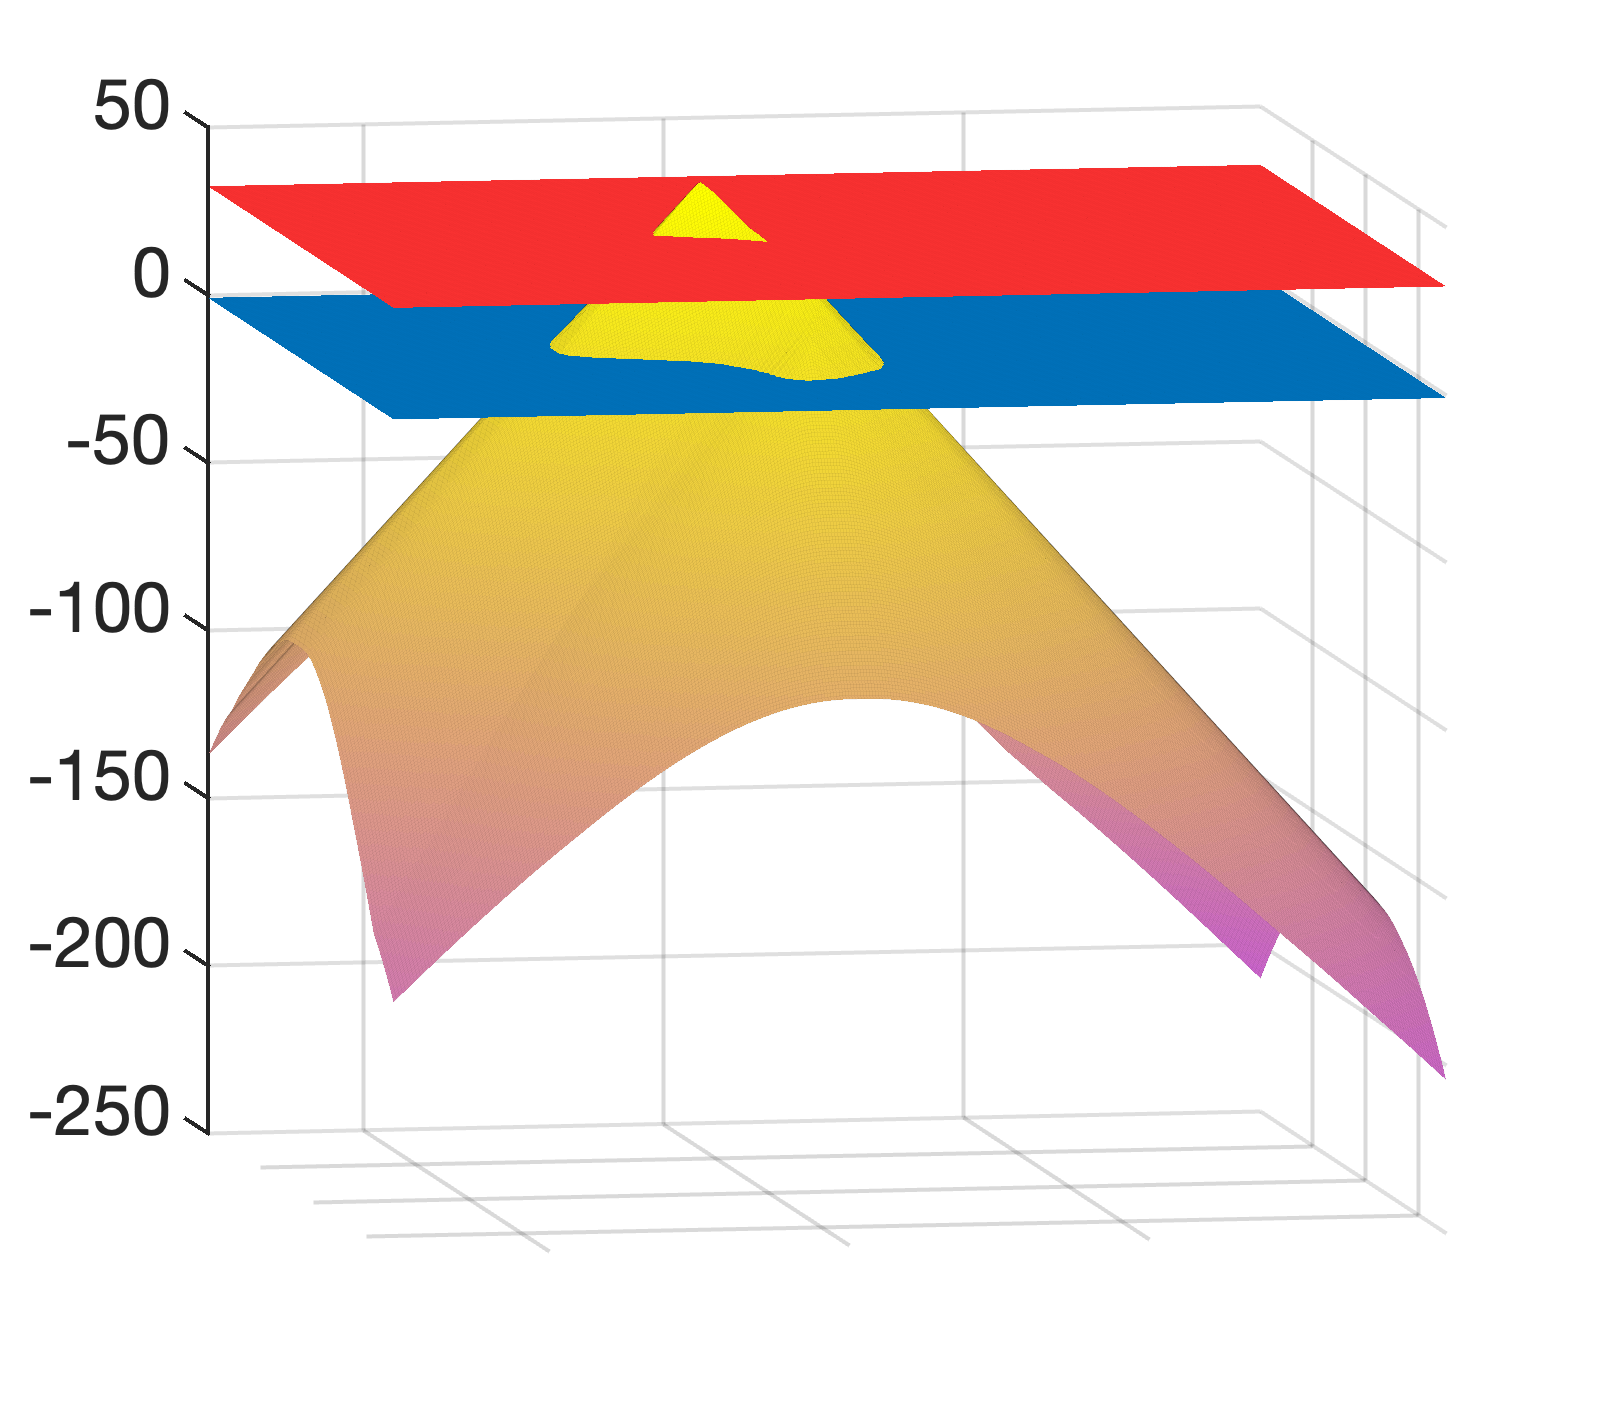
\includegraphics[width=0.24\textwidth]{../figures/learning/dist_surf/183.png}
		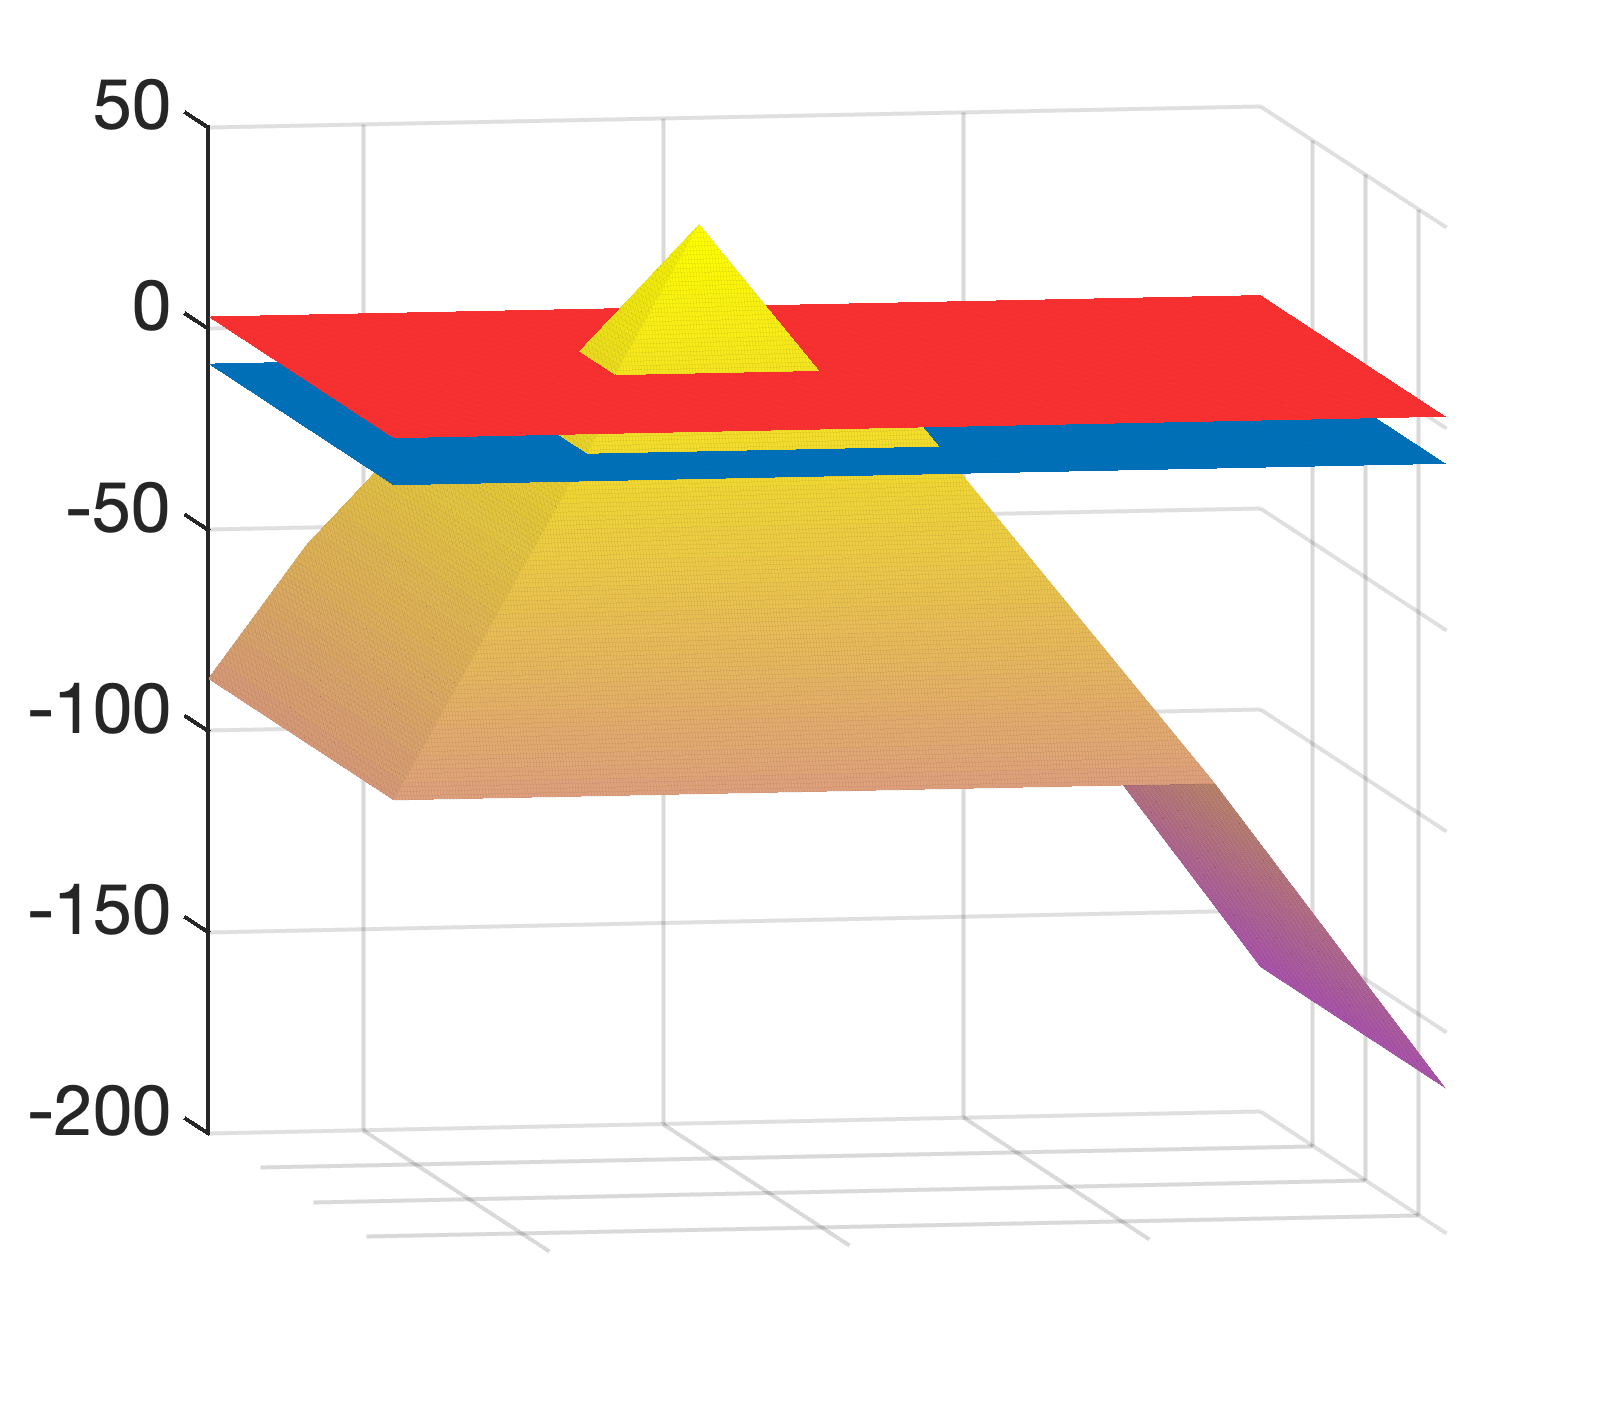
\includegraphics[width=0.24\textwidth]{../figures/learning/dist_bt_surf/183.png}\\
		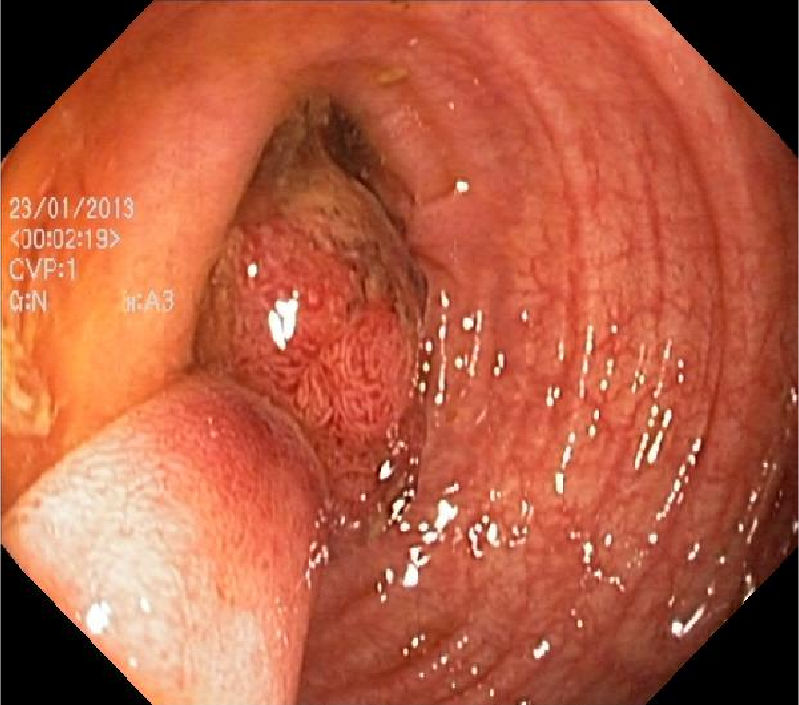
\includegraphics[width=0.24\textwidth]{../figures/learning/images/183.png}
		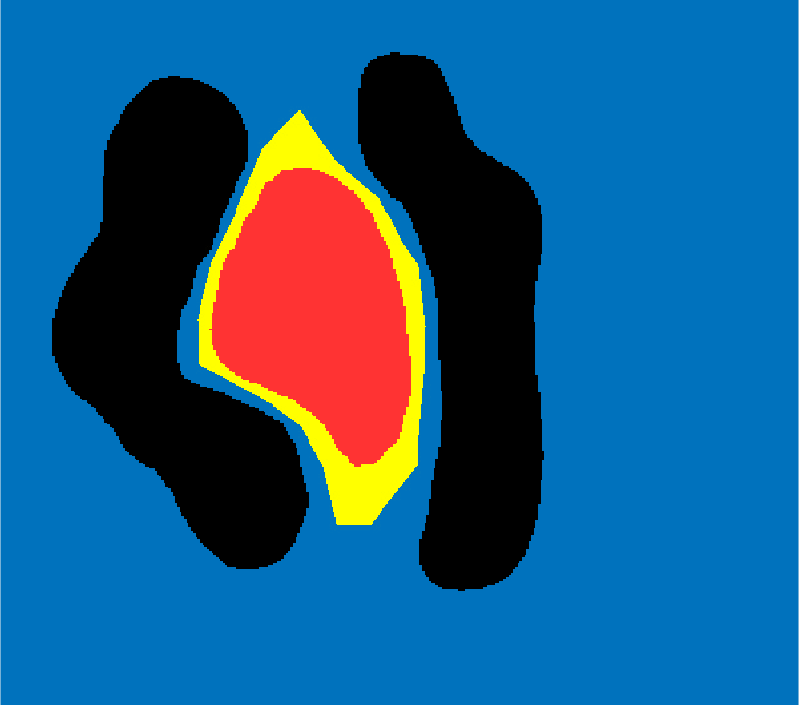
\includegraphics[width=0.24\textwidth]{../figures/learning/score_crs_marginal90/183.png}
		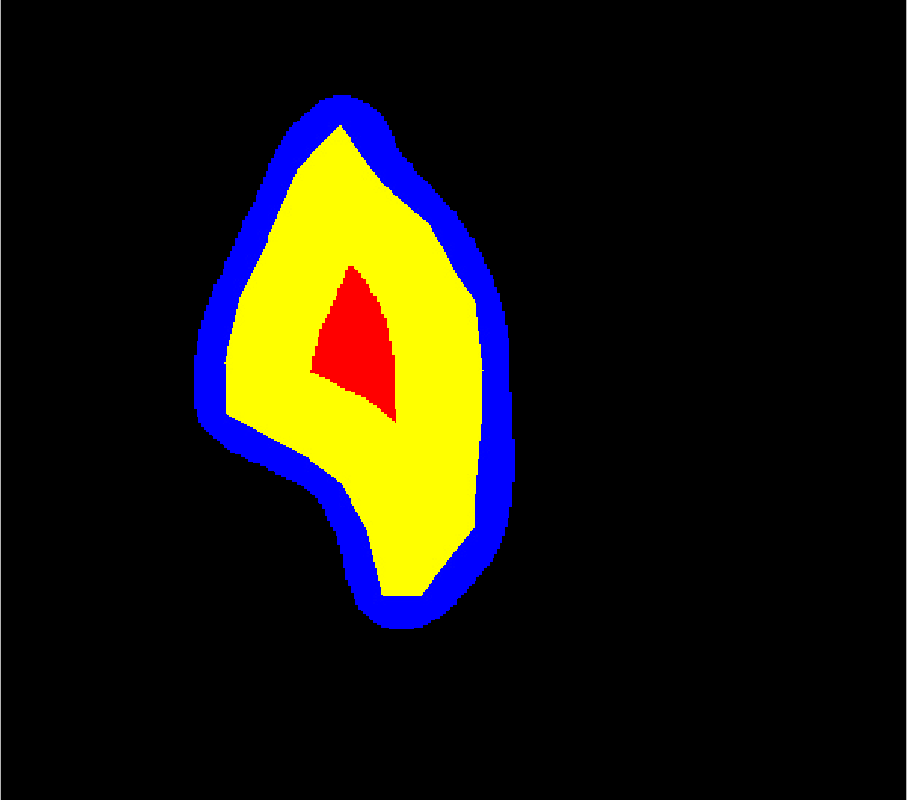
\includegraphics[width=0.24\textwidth]{../figures/learning/dist_crs_marginal90/183.png}
		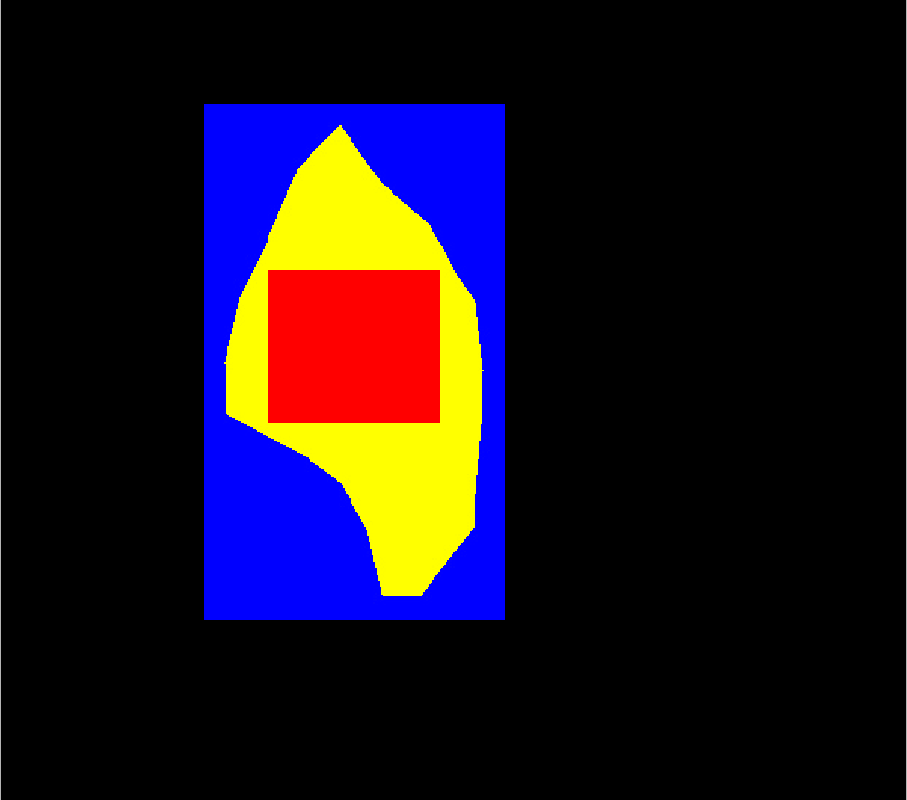
\includegraphics[width=0.24\textwidth]{../figures/learning/dist_bt_crs_marginal90/183.png}\\
		\vspace{0.5cm}
		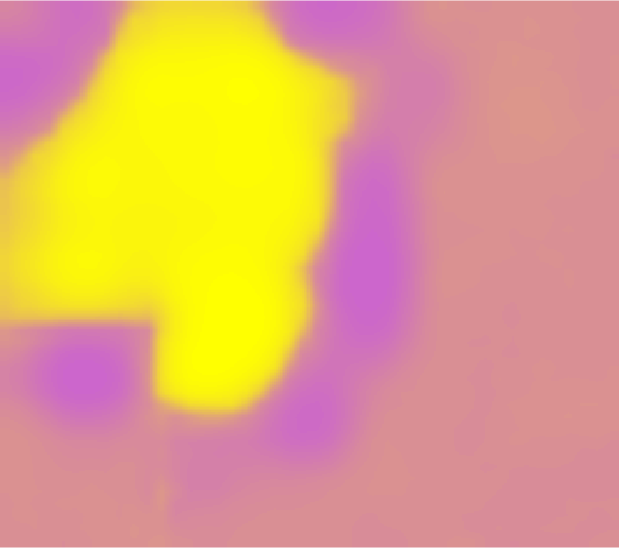
\includegraphics[width=0.24\textwidth]{../figures/learning/scores/530.png}
		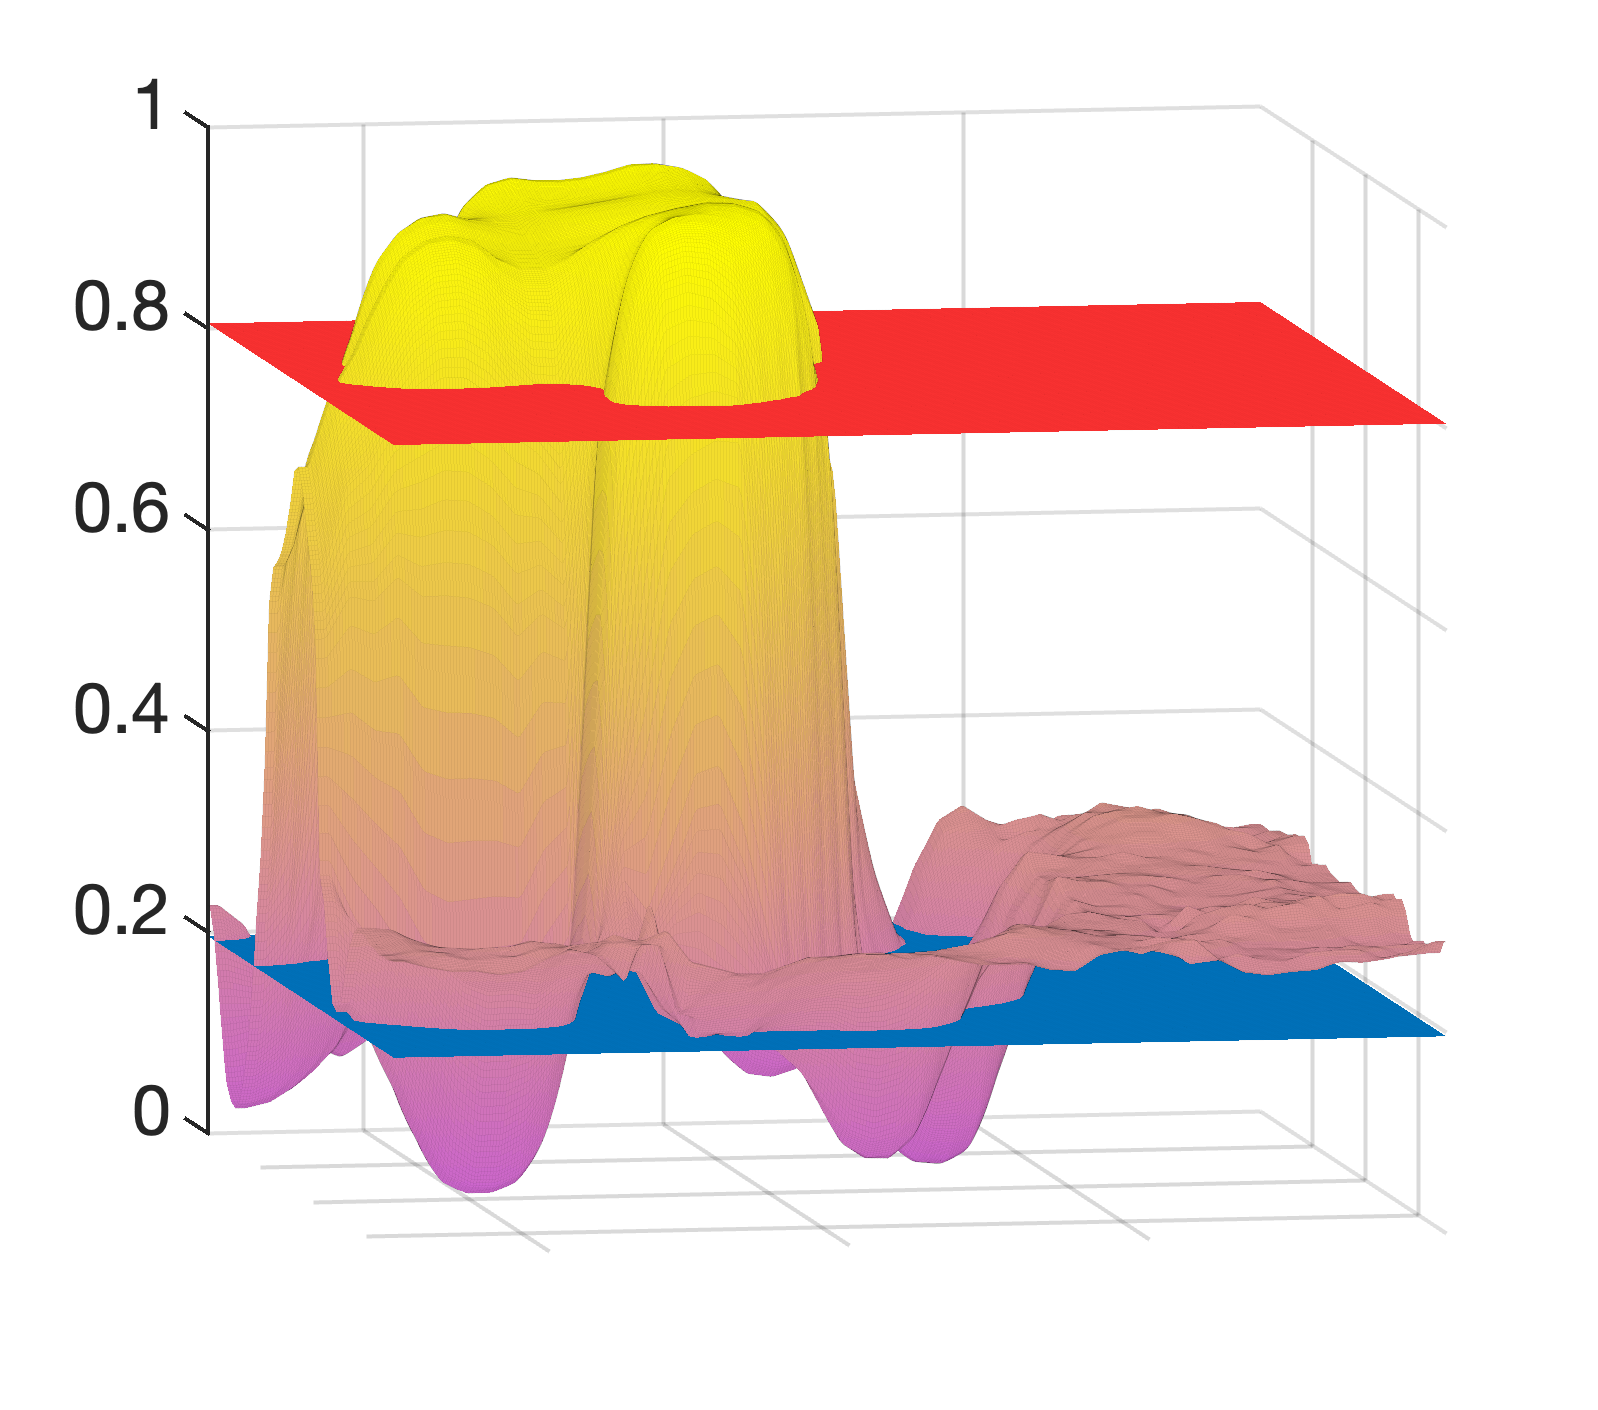
\includegraphics[width=0.24\textwidth]{../figures/learning/score_surf/530.png}	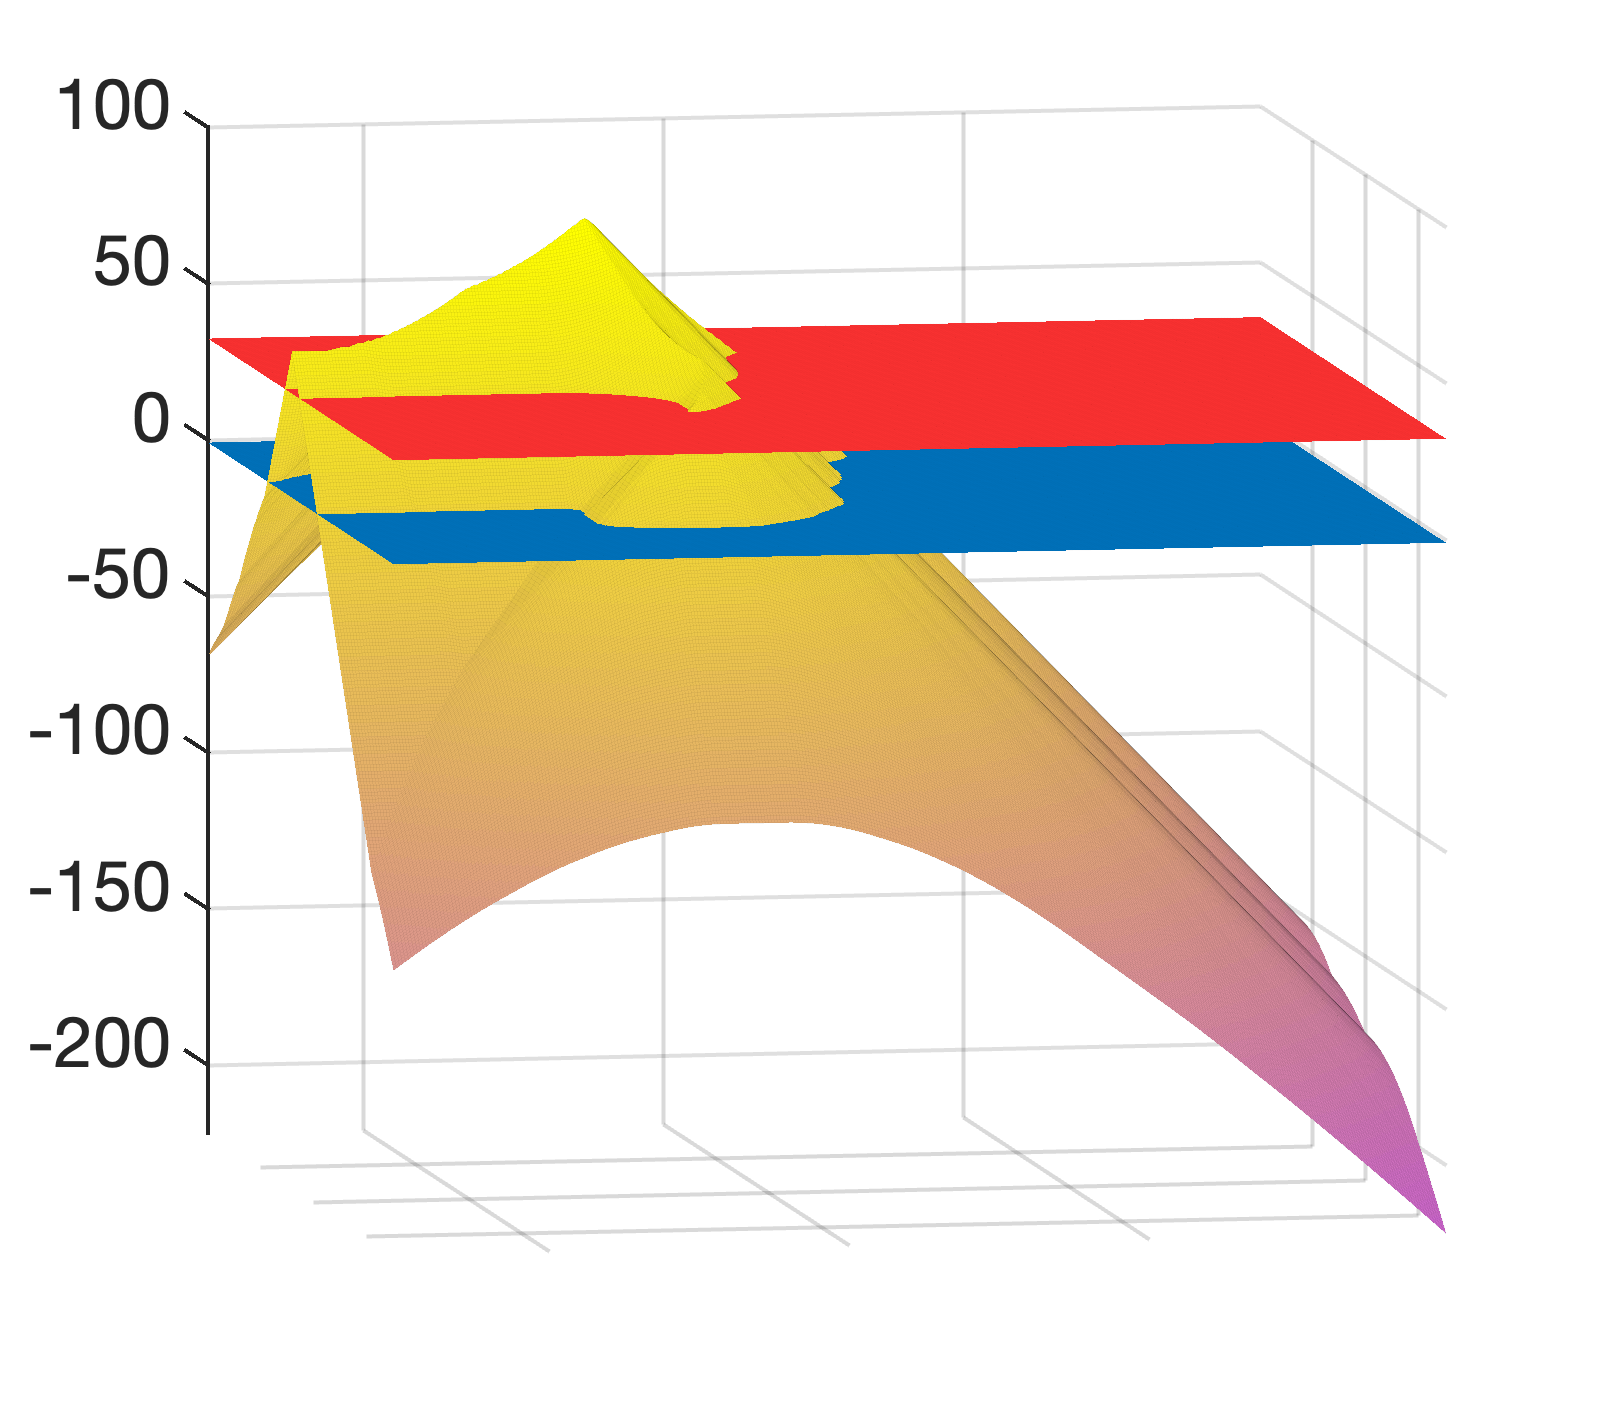
\includegraphics[width=0.24\textwidth]{../figures/learning/dist_surf/530.png}
		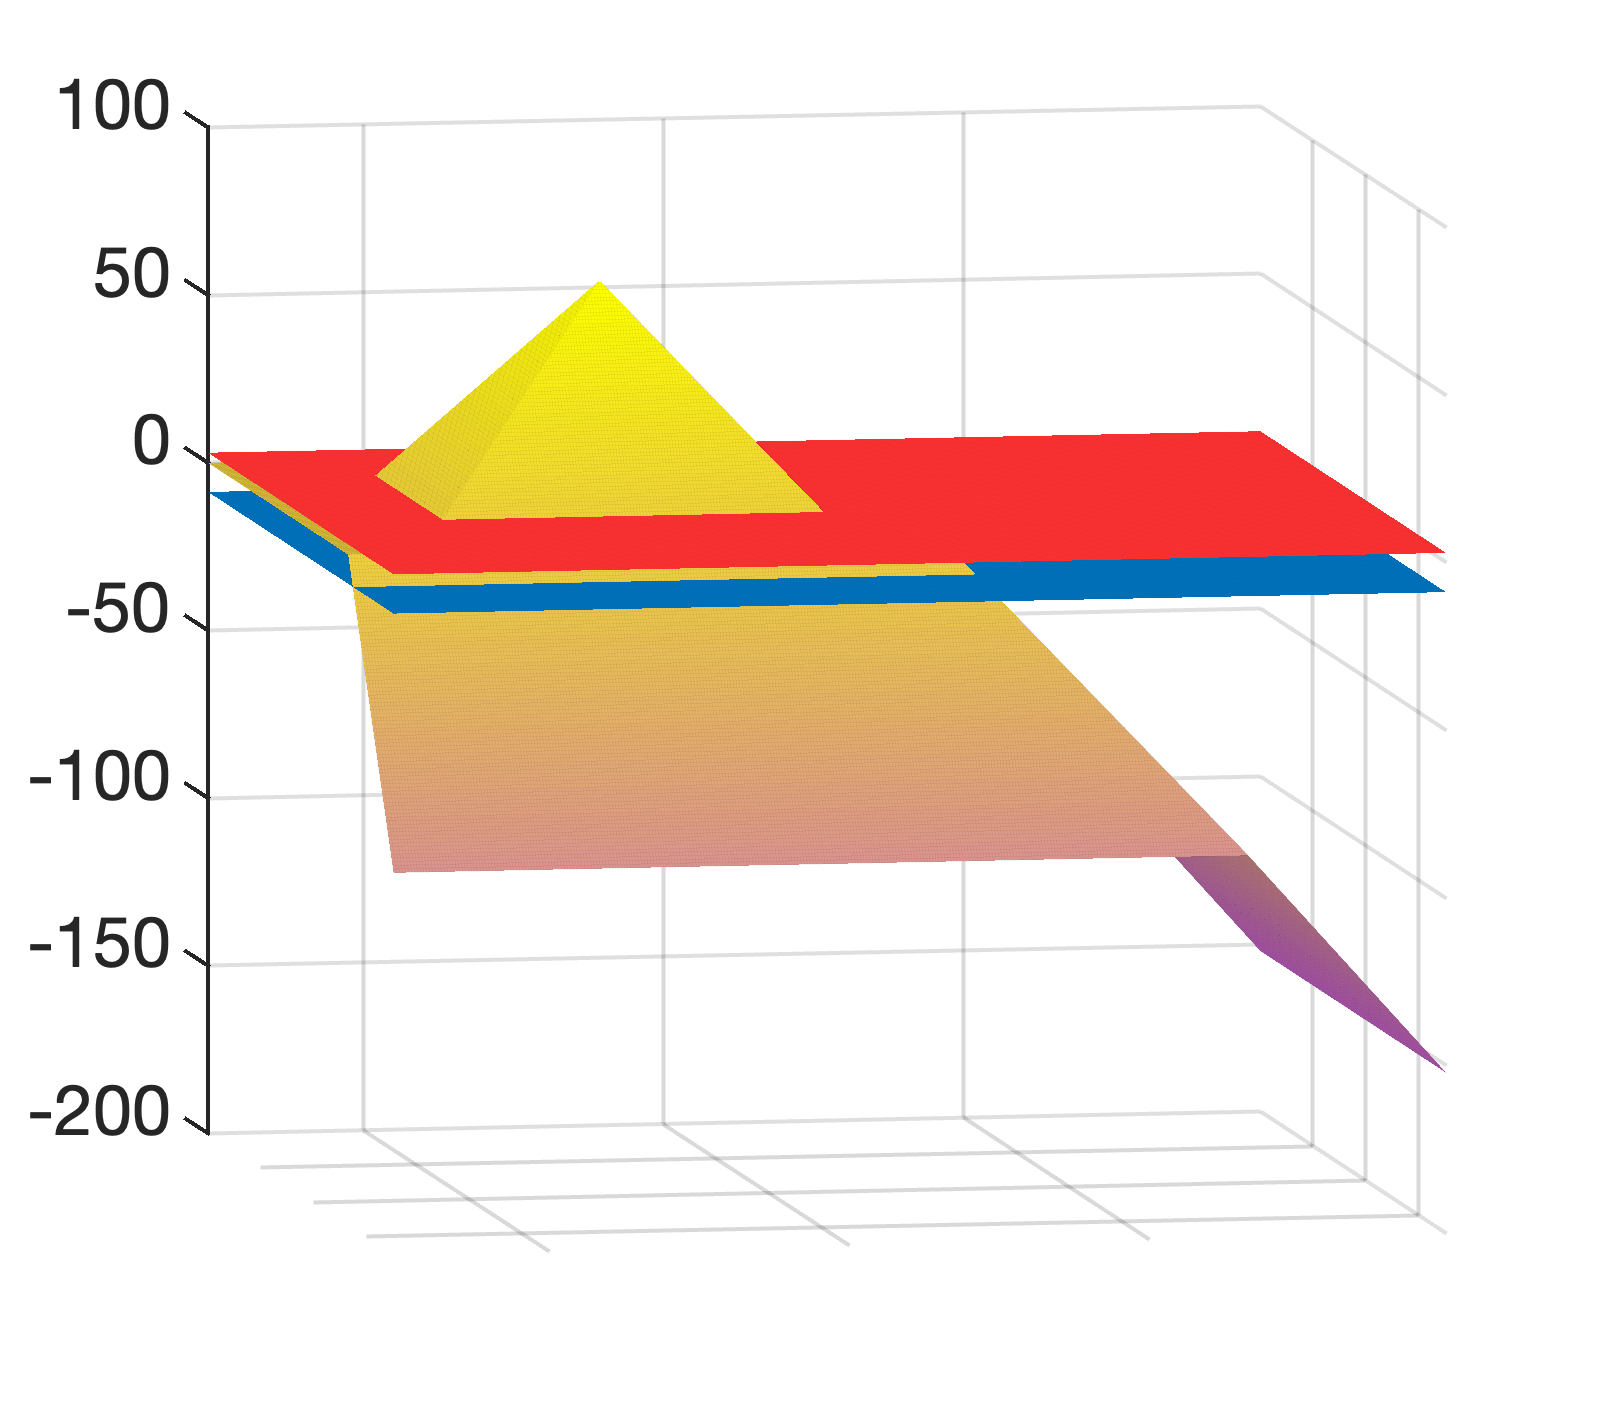
\includegraphics[width=0.24\textwidth]{../figures/learning/dist_bt_surf/530.png}\\
		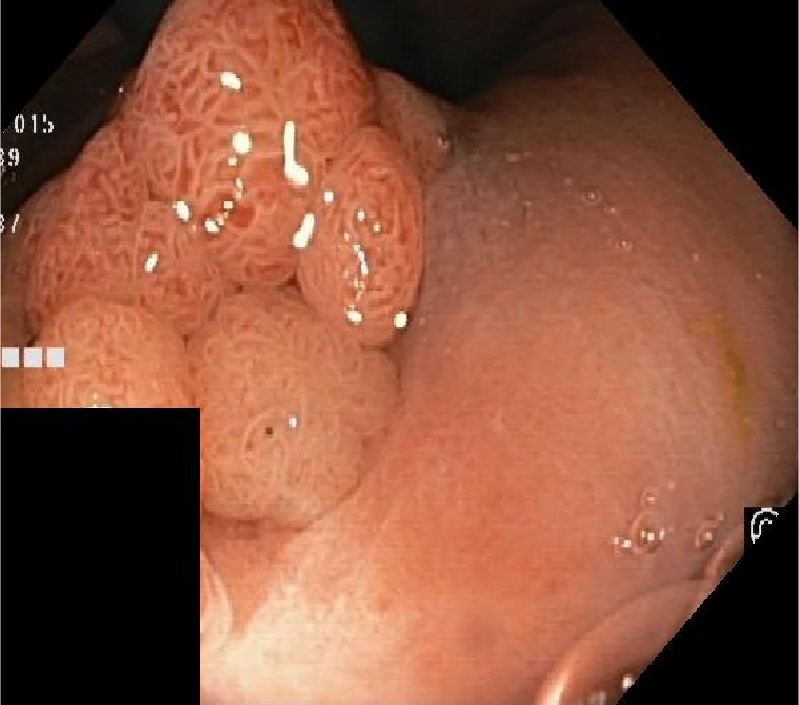
\includegraphics[width=0.24\textwidth]{../figures/learning/images/530.png}
		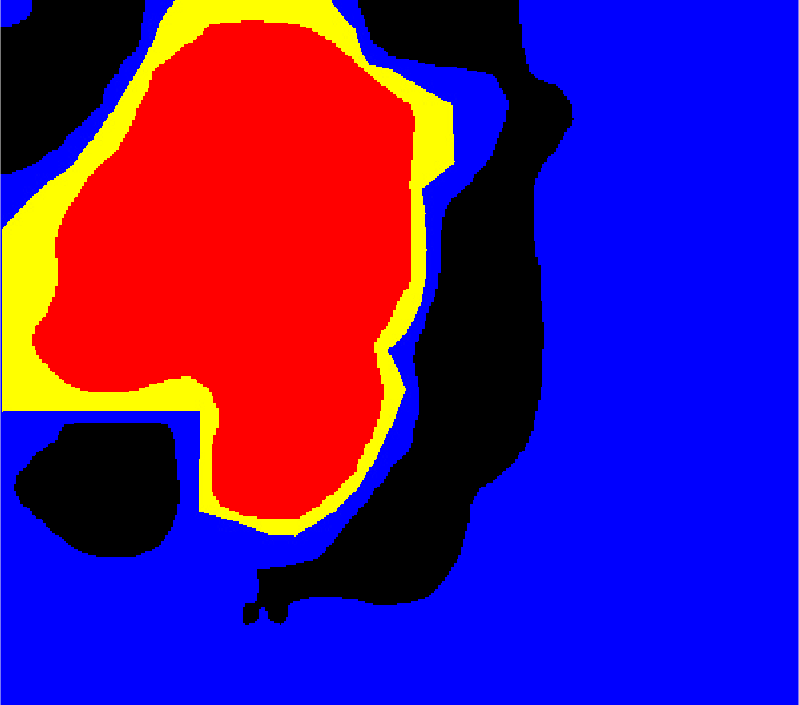
\includegraphics[width=0.24\textwidth]{../figures/learning/score_crs_marginal90/530.png}
		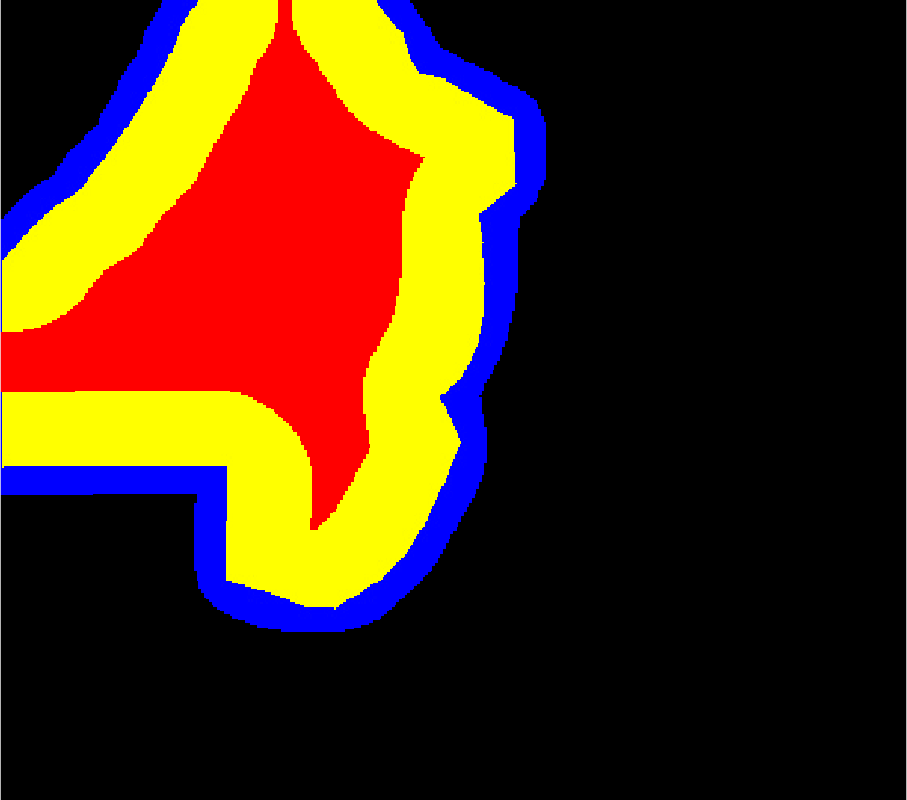
\includegraphics[width=0.24\textwidth]{../figures/learning/dist_crs_marginal90/530.png}
		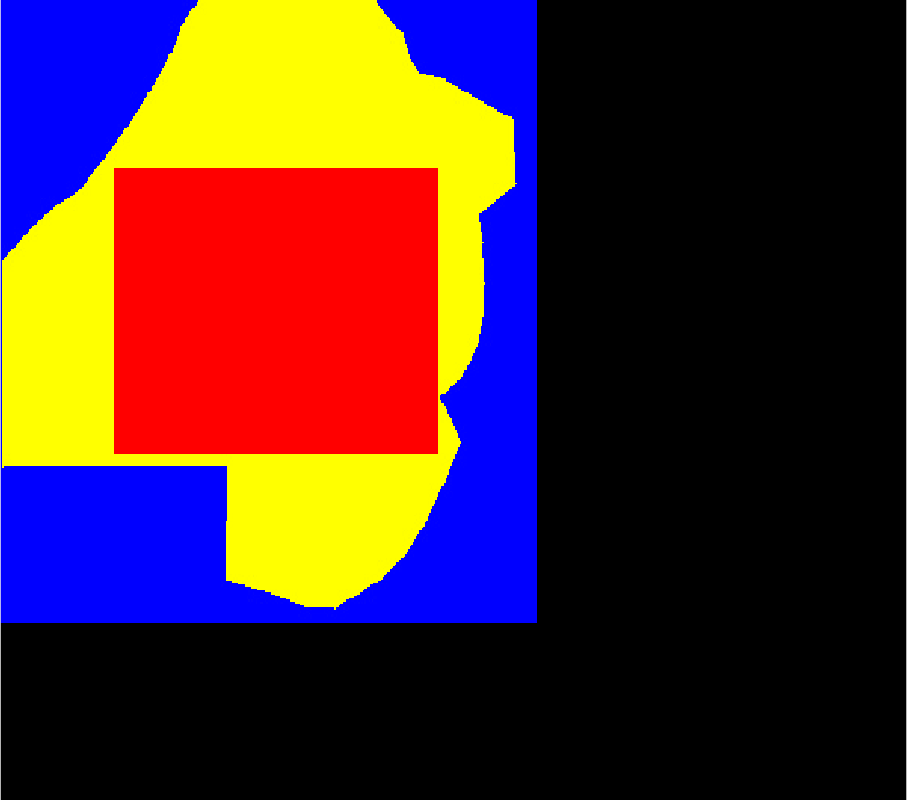
\includegraphics[width=0.24\textwidth]{../figures/learning/dist_bt_crs_marginal90/530.png}\\
		\vspace{0.5cm}
		
\includegraphics[width=0.24\textwidth]{../figures/learning/scores/754.png}
		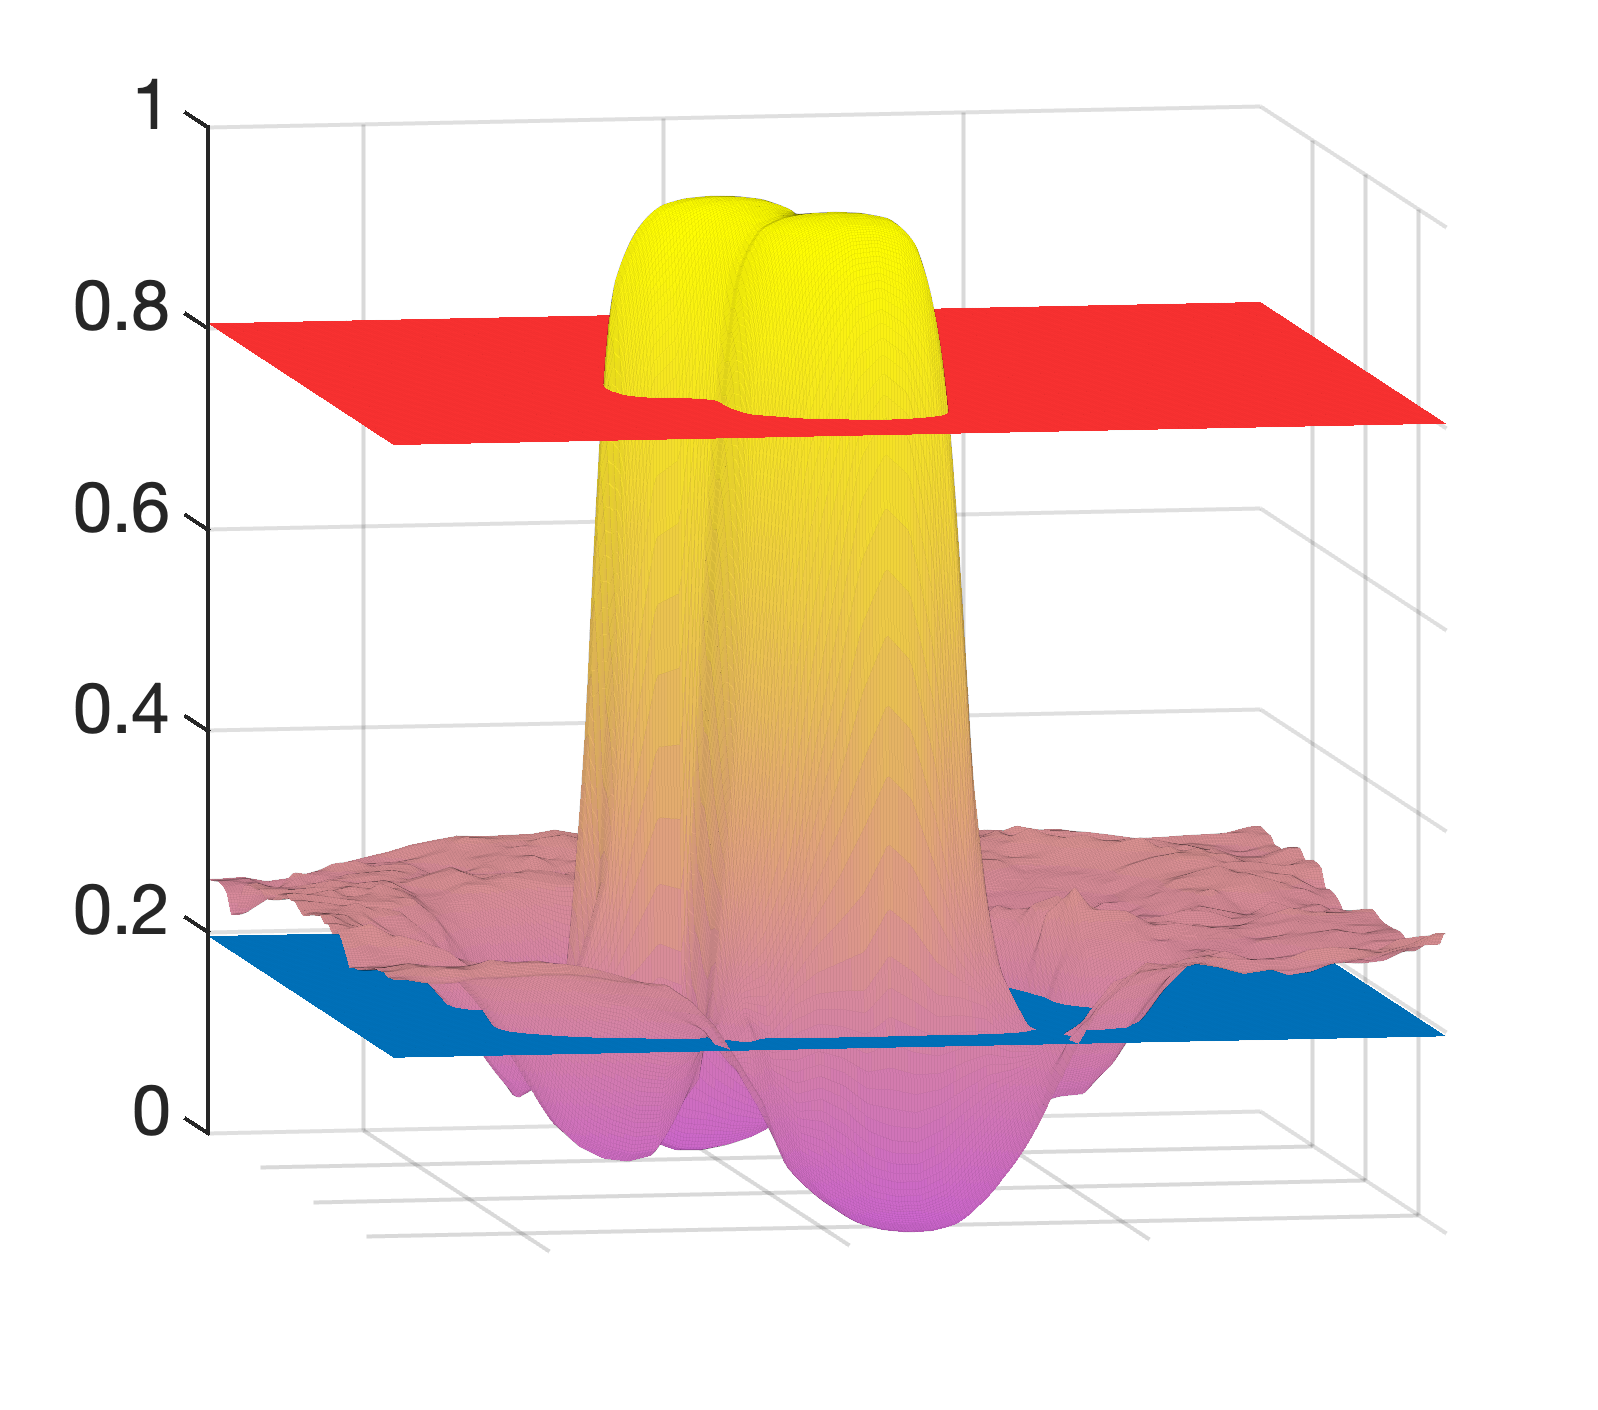
\includegraphics[width=0.24\textwidth]{../figures/learning/score_surf/754.png}	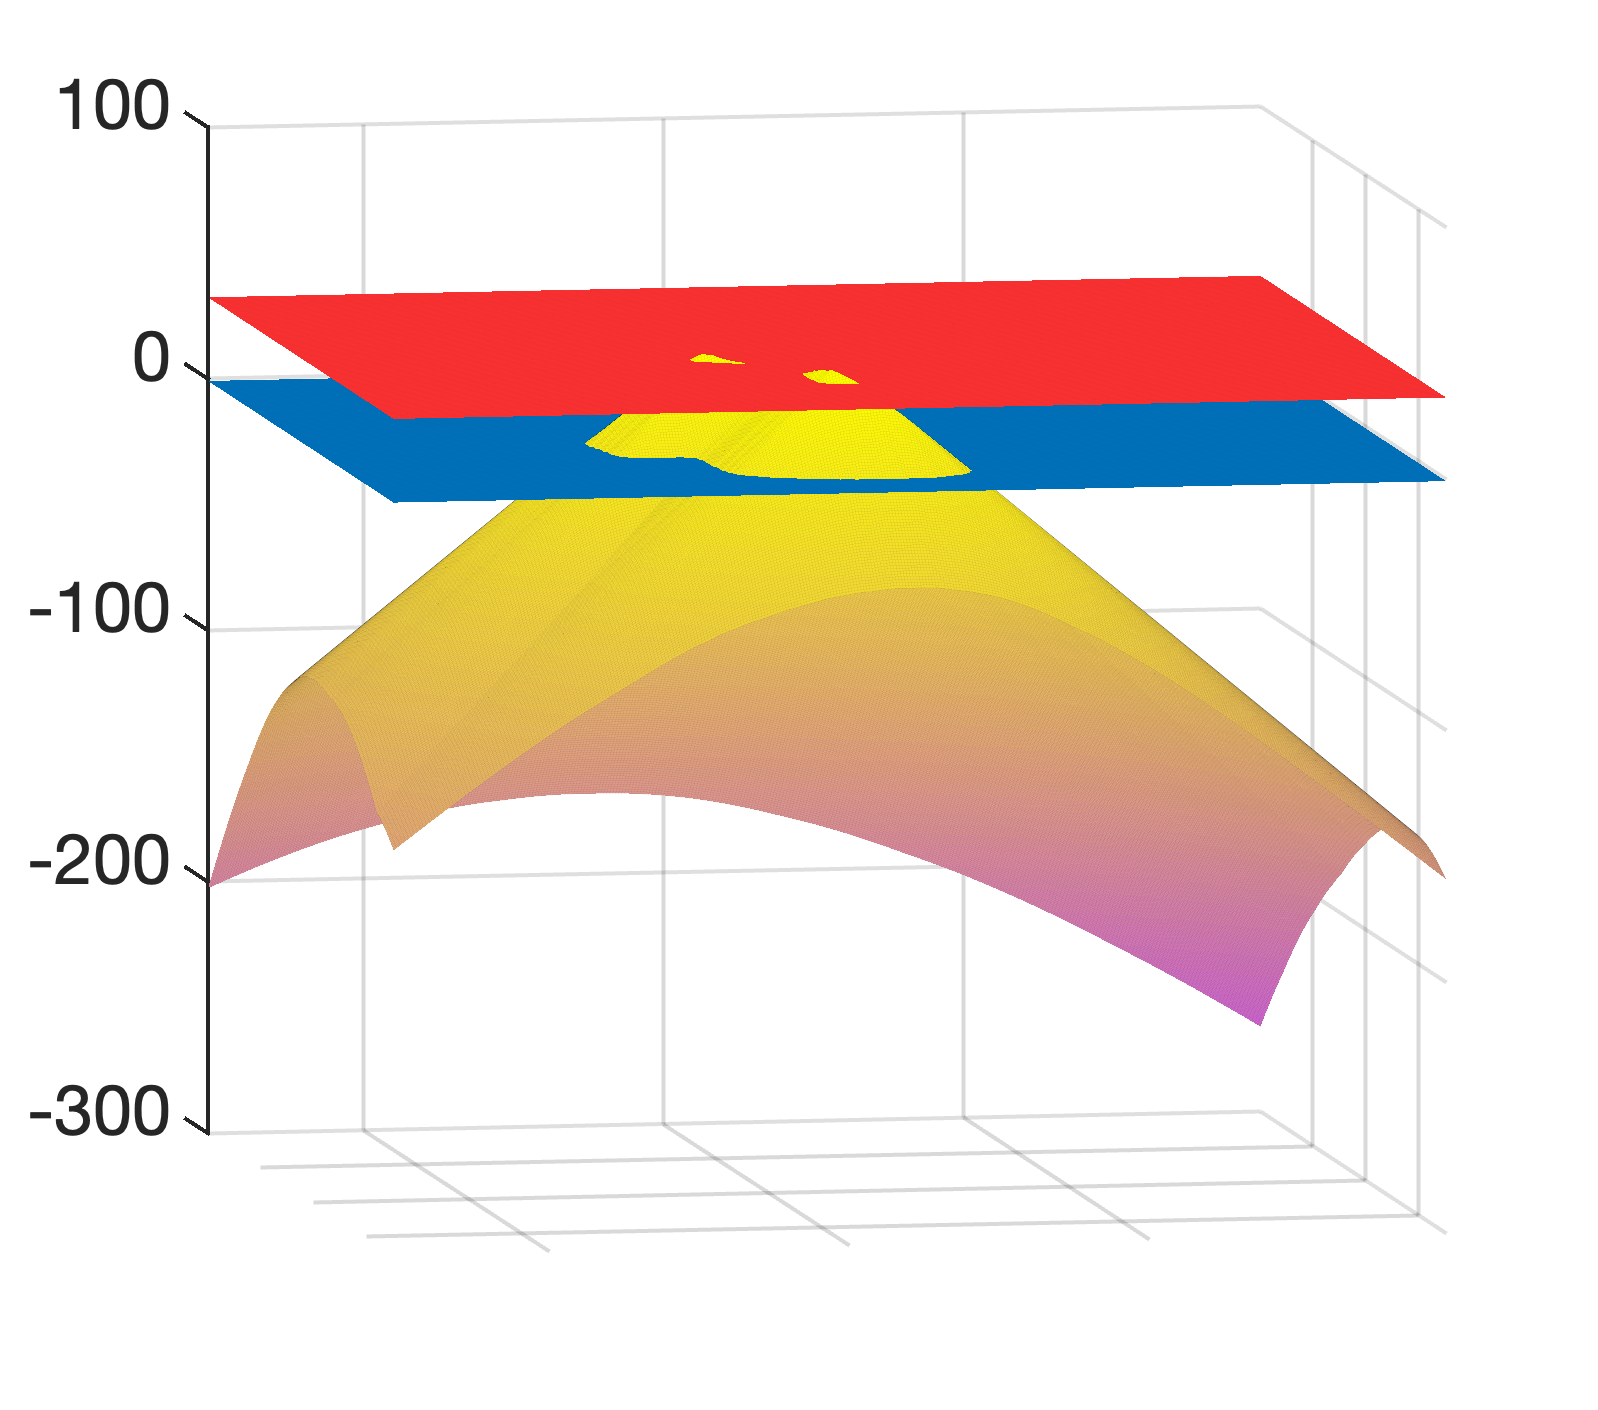
\includegraphics[width=0.24\textwidth]{../figures/learning/dist_surf/754.png}
		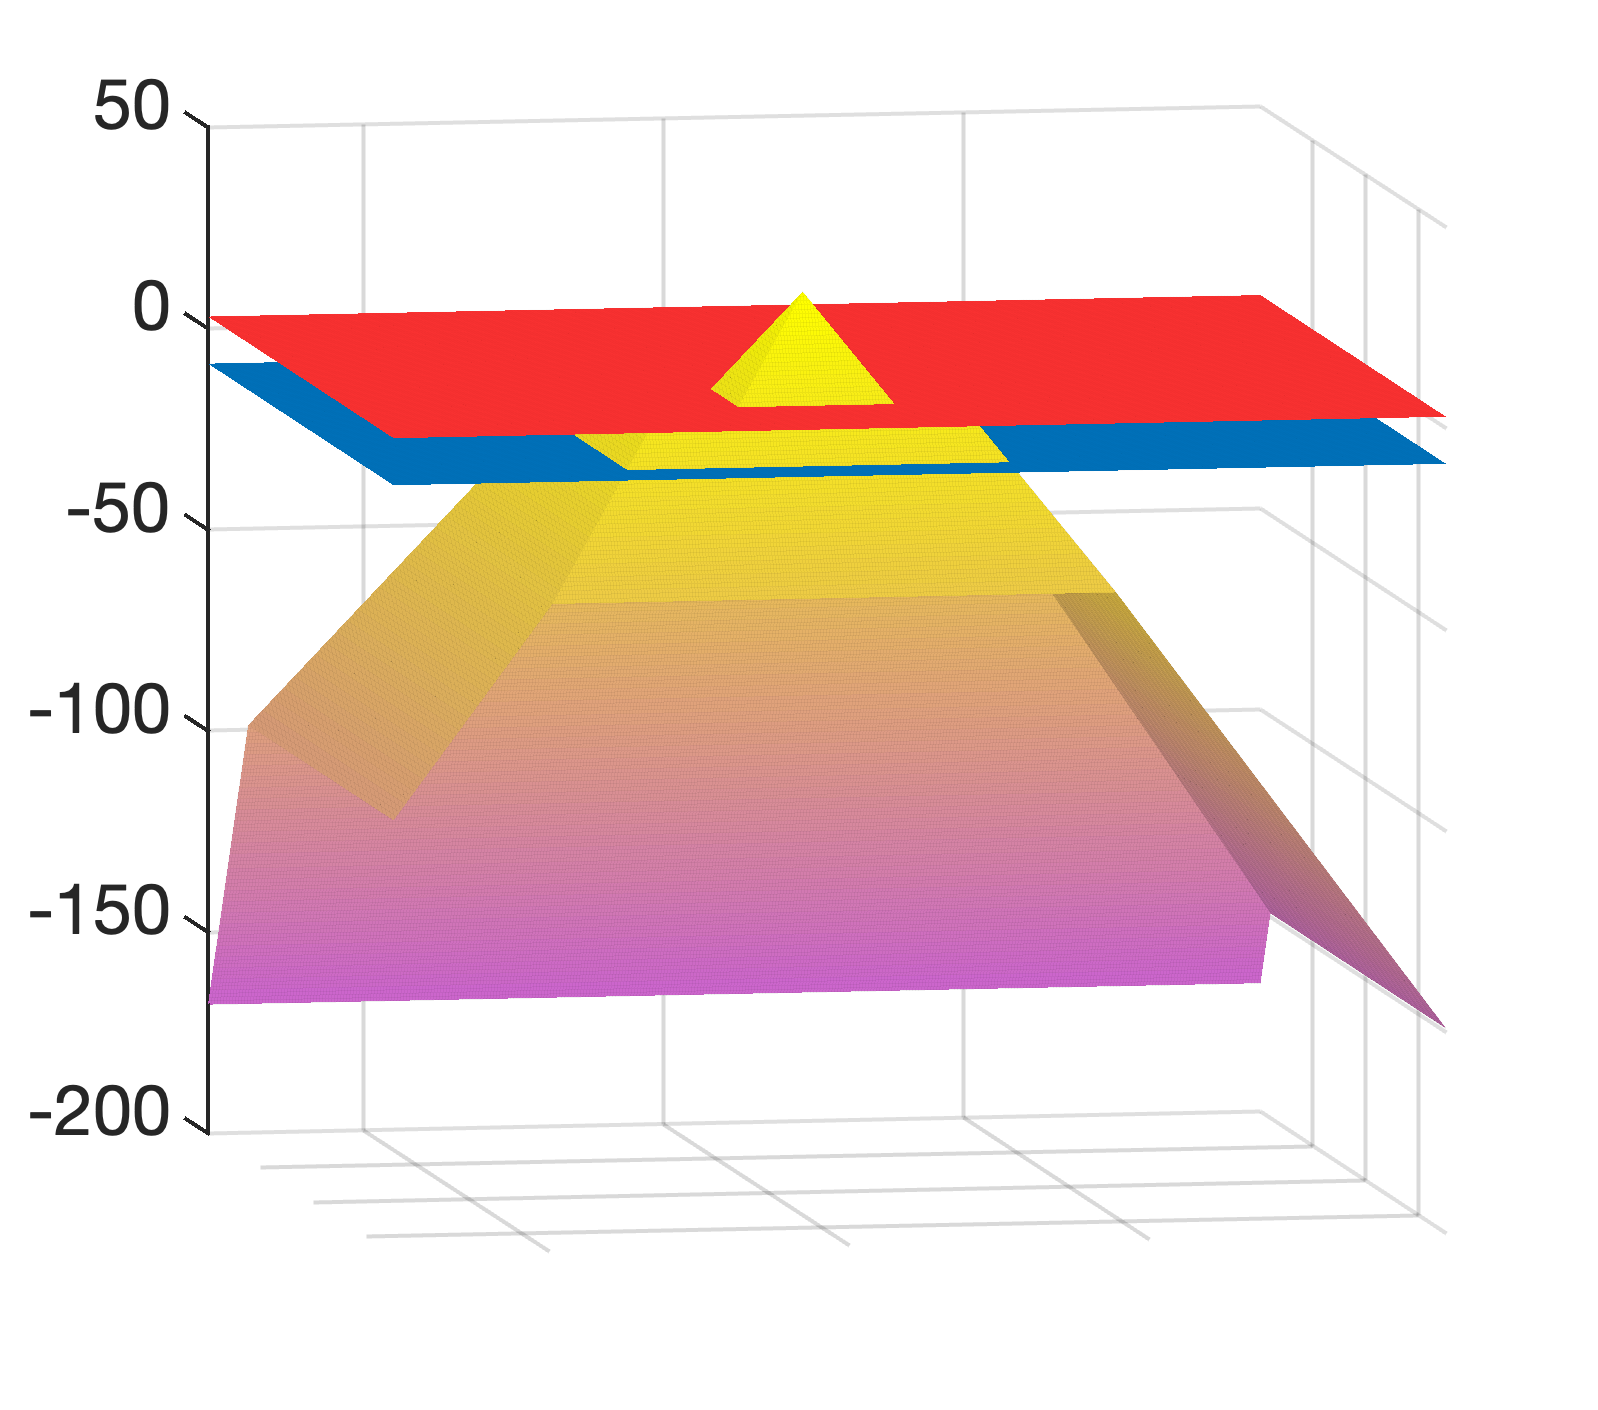
\includegraphics[width=0.24\textwidth]{../figures/learning/dist_bt_surf/754.png}\\
		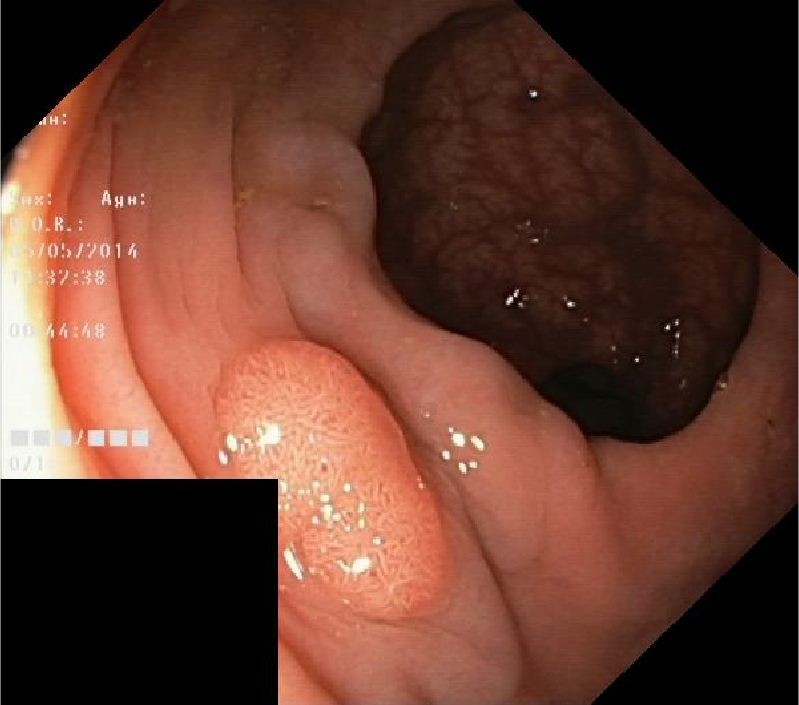
\includegraphics[width=0.24\textwidth]{../figures/learning/images/754.png}
		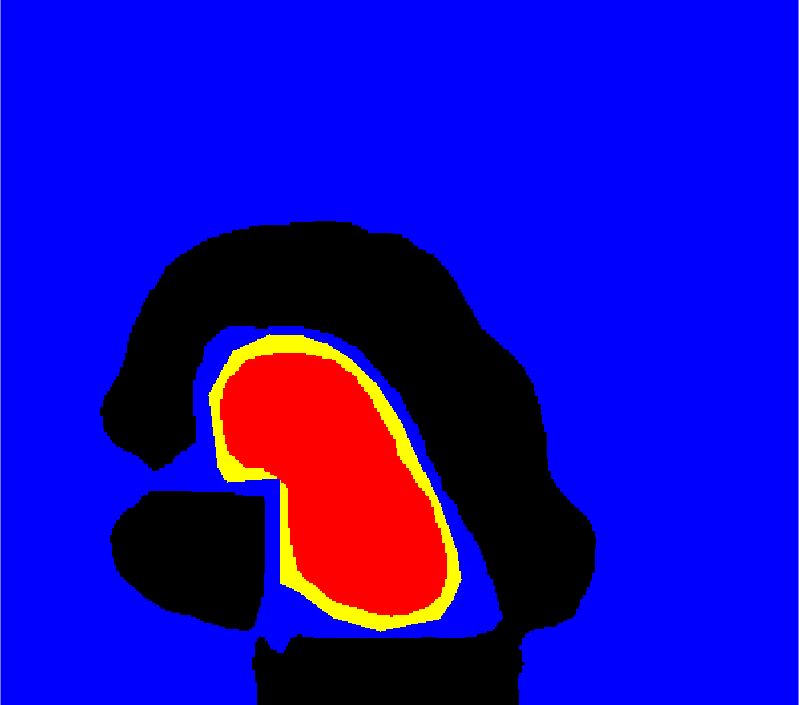
\includegraphics[width=0.24\textwidth]{../figures/learning/score_crs_marginal90/754.png}
		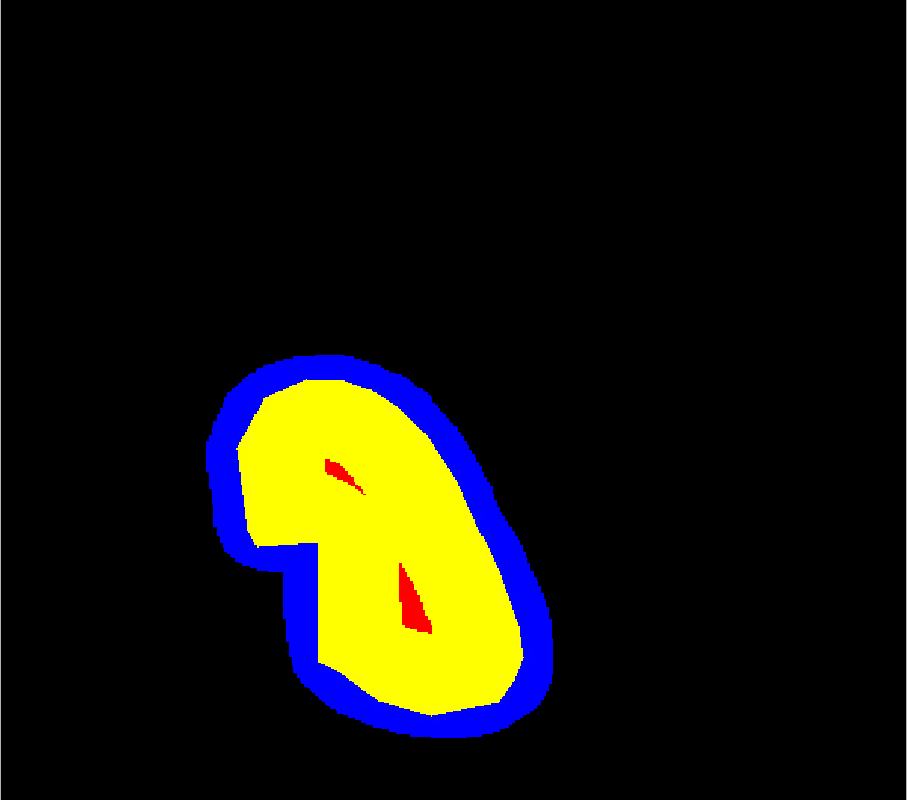
\includegraphics[width=0.24\textwidth]{../figures/learning/dist_crs_marginal90/754.png}
		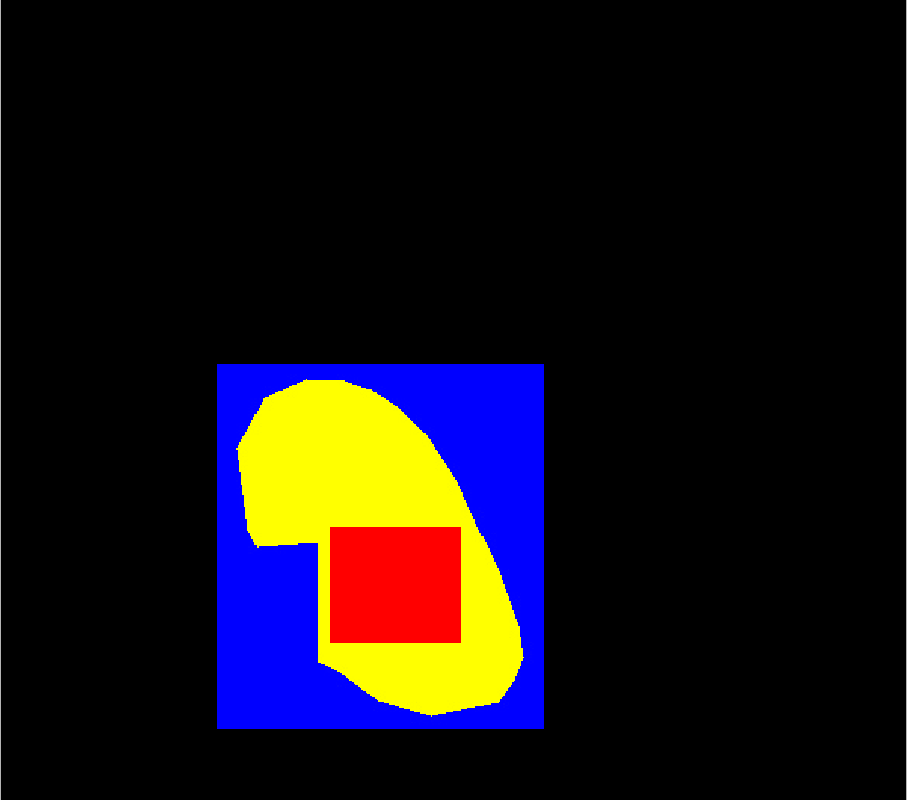
\includegraphics[width=0.24\textwidth]{../figures/learning/dist_bt_crs_marginal90/754.png}
	\end{center}
	\caption{Futher examples from the learning dataset. The layout of these figures is the same as for Figure \ref{fig:learning}.}
	\label{fig:learning3}
\end{figure}

\newpage
\subsection{Histograms of the coverage}
\begin{figure}[h!]
	\begin{center}
		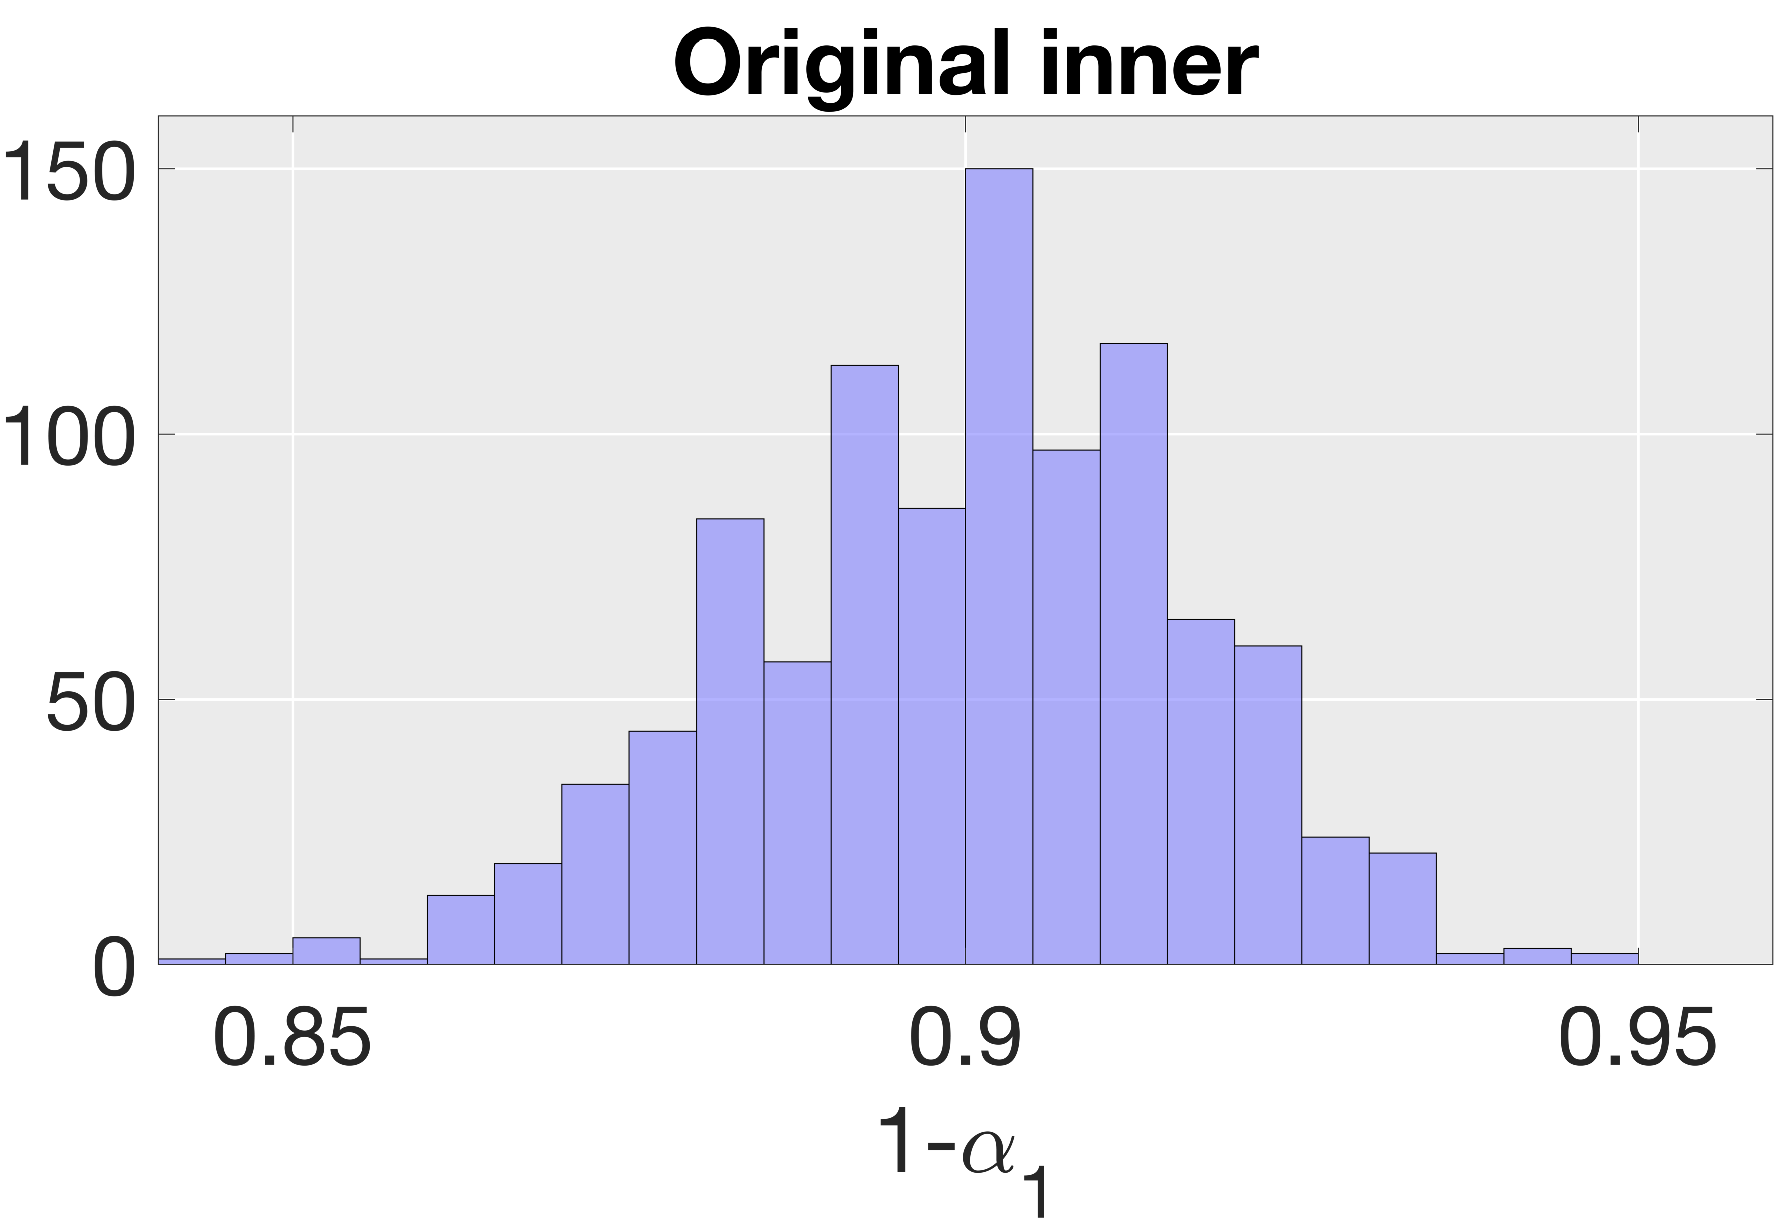
\includegraphics[width=0.32\textwidth]{../figures/validation/val_hist_orig_inner.pdf}
		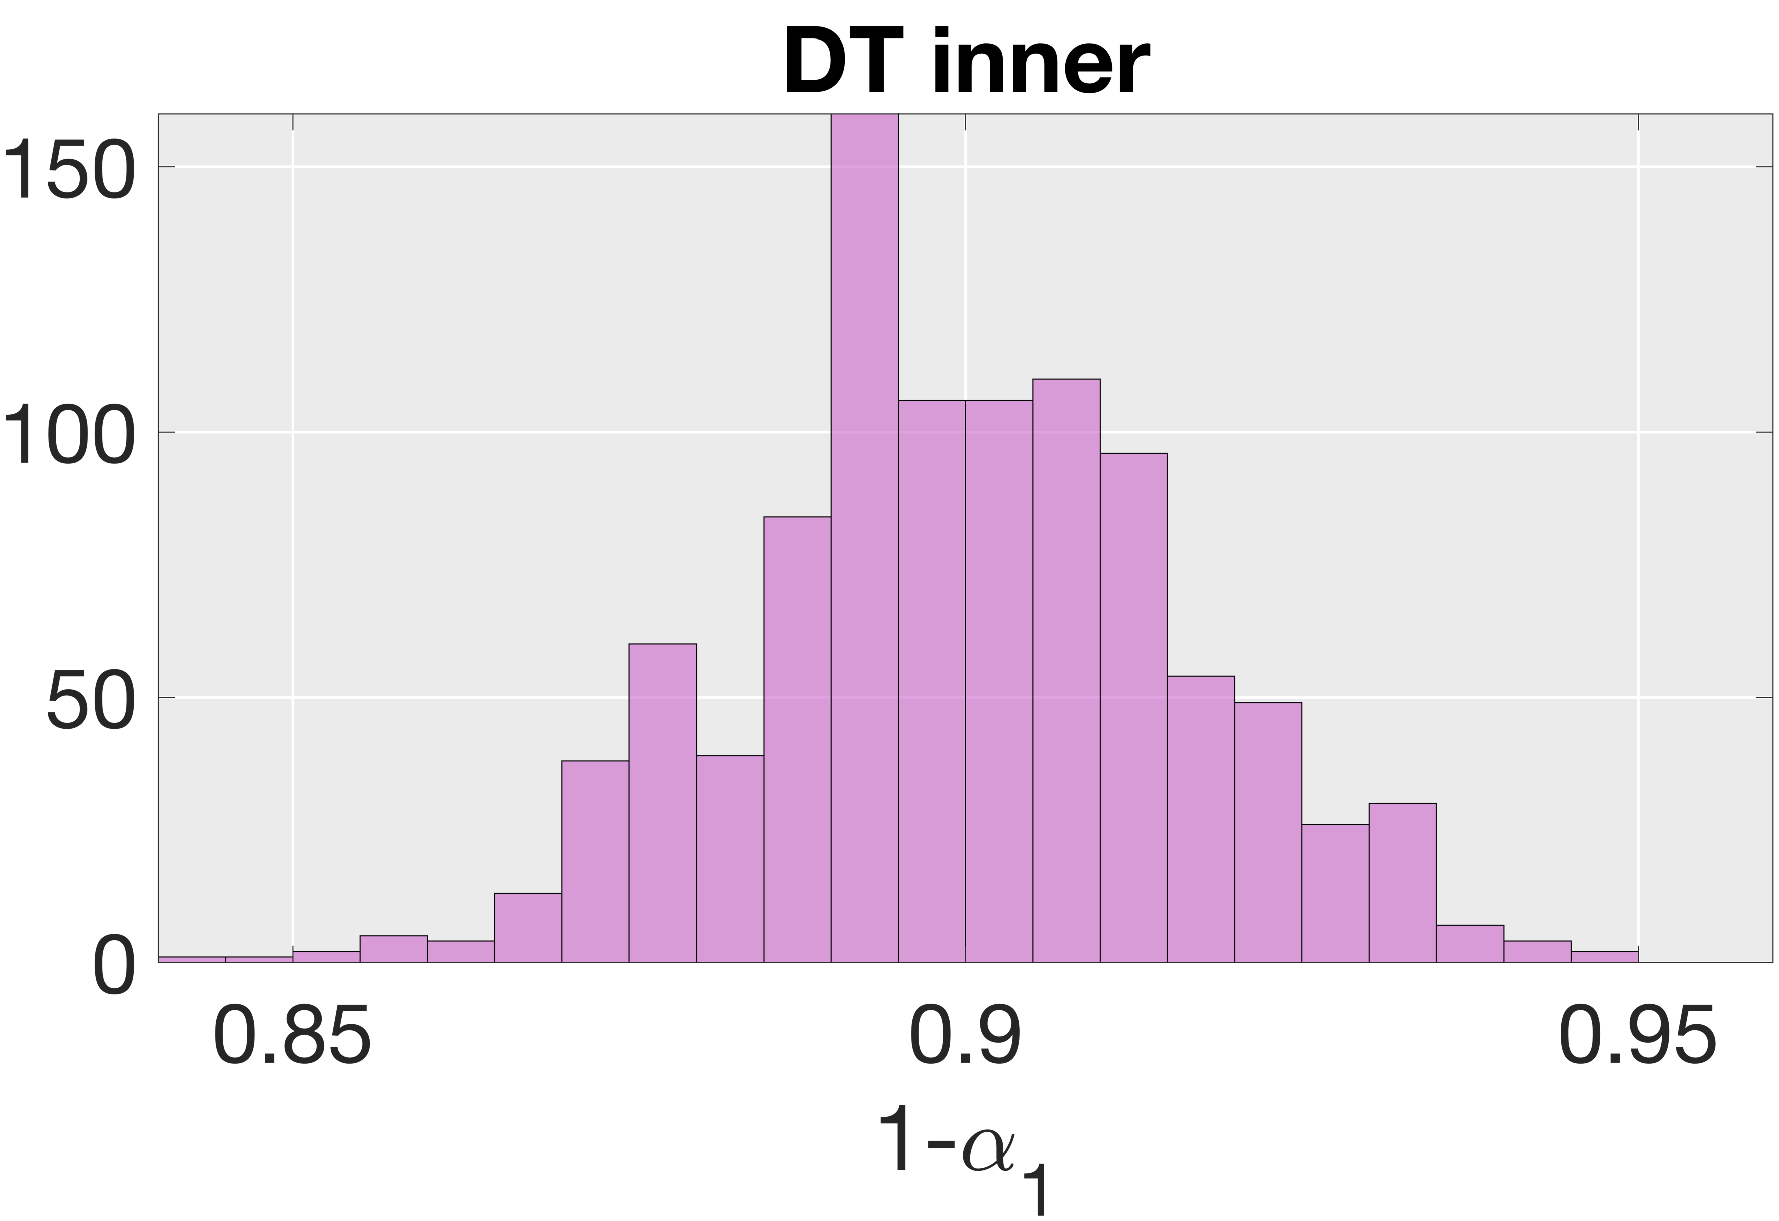
\includegraphics[width=0.32\textwidth]{../figures/validation/val_hist_dt_inner.pdf}
		\includegraphics[width=0.32\textwidth]{../figures/validation/val_hist_bt_inner.pdf}\\
		\includegraphics[width=0.32\textwidth]{../figures/validation/val_hist_orig_outer.pdf}
		\includegraphics[width=0.32\textwidth]{../figures/validation/val_hist_dt_outer.pdf}
		\includegraphics[width=0.32\textwidth]{../figures/validation/val_hist_bt_outer.pdf}
	\end{center}
	\caption{Histograms of the coverage rates obtained across each of the validation resamples for 90\% inner and outer marginal confidence sets. We plot the results for the original scores, distance transformed scores (DT) and boundary box scores (BB) from left to right. The bounding box scores are discontinuous which is the cause of the discreteness of the rightmost histogram.}\label{fig:valhist}
\end{figure}

\newpage
\subsection{Additional examples from the validation set}

